\RequirePackage { setspace}
\documentclass[12pt]{report}%tama;o de letra y tipo de documento
\usepackage[spanish]{babel}%para poder usar caracteres latinos
%\usepackage[latin1]{inputenc}%para poder usar caracteres latinos pero no funcionaba en mac
\usepackage{times}
\usepackage{tikz}
\usepackage{pgf-pie}
\usetikzlibrary{shadows}
\usepackage{hyperref}
\usepackage{multirow}
\usepackage[spanish]{babel}
\usepackage{amsmath,amsfonts}
\usepackage{amssymb}
\usepackage{pdflscape}
\usepackage{fancyhdr}
\usepackage{subfigure}
\usepackage{enumerate}
\usepackage{setspace}%configuraciones de interlineado
\usepackage{colortbl}
\usepackage{float}%CONFIGURACIONES PARA IMAGEN
\usepackage{pdfpages}
\usepackage{lettrine}
\usepackage[spanish]{layout}
\usepackage{graphicx}%imagenes
%\usepackage{cite}%referencias
\usepackage[papersize={21.59cm,27.94cm},left=3cm,right=2.54cm,top=2.54cm, bottom=3cm]{geometry}%defino tamaño de pagina y margenes
\usepackage{enumitem}
\usepackage{setspace}
\usepackage{hyperref}
\setlist{nolistsep}
\usepackage{chngcntr}
\counterwithout{footnote}{chapter}
\usepackage{cite}
\makeatletter
\usepackage[hang,flushmargin]{footmisc}
\renewcommand\@makefntext[1]{\leftskip=2em\hskip-2em\@makefnmark#1}%referencias
\makeatother

\hypersetup{pdfborder={0 0 0}}%algo de los margenes
\graphicspath{ {imagenes/} }%indica que las imagenes estan en la  carpeta con ese nombre

%-----------------------------------INICIA DOCUMENTO---------------------------------------------------------------------------
\begin{document}%inicia docmento

%-----------------------------------CARATULA---------------------------------------------------------------------------
\begin{center}%centra
\textbf{%texto en negrita
UNIVERSIDAD DE EL SALVADOR} \\ 
FACULTAD MULTIDISCIPLINARIA ORIENTAL \\%salto de linea
DEPARTAMENTO DE INGENIERÍA Y ARQUITECTURA\\ 
 \vspace{1cm}%le da un espacio de 1cm entre elementos
 
 %codigo para insertar una imagen
\begin{figure}[h!]
	 \centering
	 
\includegraphics[width=4cm, height=4cm]{minerva1.png}
	 \label{fig:minerva1}
 \end{figure}
 
\vspace{1cm}

\textbf{TRABAJO DE GRADO: }\\

“DESARROLLO DE UN PROTOTIPO PARA LA ENSEÑANZA DE LENGUA DE SEÑAS POR MEDIO DE UN TUTOR INTERACTIVO PARA LA ESCUELA DE EDUCACIÓN ESPECIAL "SAN FRANCISCO DE ASÍS", SAN FRANCISCO GOTERA, DEPARTAMENTO DE MORAZÁN" \\

\vspace{1cm}

\textbf{PARA OPTAR AL TÍTULO DE: }\\    
\textbf{INGENIERO DE SISTEMAS INFORMÁTICOS}\\   
\vspace{1cm}

\textbf{PRESENTADO POR: }\\                                          
DÍAZ ORELLANA, REBECA ABIGAIL  \\
LAZO CRUZ, KAREN BEATRIZ  \\
NOLASCO ARGUETA, CINDY JANETH \\
\vspace{1cm}

\textbf{DOCENTE ASESOR:} \\
ING. LUDWIN ALDUVI HERNÁNDEZ VÁSQUEZ \\ 
\vspace{1cm}

\textbf{CIUDAD UNIVERSITARIA ORIENTAL, JULIO 2019.}\\
\textbf{SAN MIGUEL, EL SALVADOR, CENTRO AMÉRICA.} \\
\end{center}

\thispagestyle{empty} % para que no se numere esta pagina
\newpage%salto de linea a otra Pag


%-----------------------------------INDICE---------------------------------------------------------------------------
\tableofcontents % indice de contenidos
\thispagestyle{empty}
\newpage
%-----------------------------------INDICE DE IMAGENES---------------------------------------------------------------------------

\listoffigures
\thispagestyle{empty}
\newpage
%===================INDICE DE TABLAS---------------------------------------
\listoftables
\thispagestyle{empty}
\newpage

 \setlength{\parindent}{0.5cm}%sangria de primer parrafo
 \doublespacing%Sigifica que hay doble espacio de interlineado
 %\setlength{\parskip}{0.3 cm}%espacio entre parrafo
% \renewcommand{\baselinestretch}{2}%espacio entre parrafos

\textbf{ Introducción}

Hoy en día la tecnología está agilizando, optimizando y perfeccionando muchas de las actividades en nuestro día a día, este cambio puede notarse en el proceso educativo, en donde el modelo educativo tradicional ha sido mejorado drásticamente, siendo hoy, los recursos tecnológicos parte vital de ella. Uno de los principales avances de la tecnología en la educación ha sido la integración de diversos grupos sociales, excluidos por diversas discapacidades, entre estos se encuentran las personas con discapacidad auditiva, quienes necesitan recibir educación especial para el aprendizaje de la lengua de señas.

Existen muchas organizaciones que brindan diversos servicios a niños, jóvenes y adultos sordos, o con pérdida auditiva, entre esos servicios se encuentra la enseñanza de la lengua de señas. 

La lengua de señas o lengua de signos es un lenguaje natural de expresión y configuración gesto-espacial y percepción visual, gracias a la cual, las personas con discapacidad auditiva pueden establecer un canal de comunicación con su entorno social, ya sea conformado por otros individuos sordos o por cualquier persona que conozca la lengua de señas empleada.  \footnote{ Lengua de señas, glosario. Espacio Logopedico, Recuperado de https://www.espaciologopedico.com}%referencia a pie de pagina

La mano humana constituye un medio de comunicación en estas personas con deficiencia auditivas, pudiendo expresar letras, palabras o con la ayuda de gestos pueden expresar emociones o ideas. 

Explicado lo anterior se propone el desarrollar un prototipo para la enseñanza de lengua de señas por medio de tutor interactivo para la Escuela  de Educación Especial “San Francisco de Asís", San Francisco Gotera, departamento Morazán. 

%-----------------------------------CAPITULO1---------------------------------------------------------------------------
\newpage
\chapter{Estudio Preliminar}%añade capitulo
\newpage

\newpage
\section{Planteamiento del Problema}
\subsection{Definición del tema}
Desarrollo de un Prototipo para la enseñanza de lengua de señas por medio de un tutor interactivo para la Escuela de Educación Especial “San Francisco de Asís", San Francisco Gotera, Departamento de Morazán.

\subsection{Situación Problemática}%es como subtitulo
La comunicación es la acción consciente de intercambiar información entre dos o más participantes con el fin de transmitir o recibir significados a través de un sistema compartido de signos y normas semánticas. \footnote{ Gutierrez, A. La comunicación, Calameo. Recuperado de https://en.calameo.com}
Una de las principales formas de comunicación es la verbal la cual es aquella en la que usamos las palabras, los signos sonoros o los auditivos. Sin embargo, estas condiciones no son ecuánimes en todos, ya que muchos por defectos en su nacimiento como también por malformaciones congénitas o incluso por accidentes durante su vida, no tienen la capacidad plena de hacer uso de los cinco sentidos que permiten la percepción con el mundo, por lo que se requiere la aplicación eficaz y universal de distintos mecanismos de adaptación que permitan subsanar levemente esta carencia. 

Si hablamos de la pérdida auditiva, el mecanismo utilizado para lograr intercambiar información y establecer una comunicación es la lengua de señas o de signos, pero es aquí donde logramos ver la necesidad de medidas para la enseñanza de esta lengua, en El Salvador existen actualmente 28,526 personas que tienen alguna discapacidad auditiva, más de 6,000 personas sordas, y aproximadamente 19,000 personas que tienen pérdida de audición hipoacusia, o disminución de la capacidad auditiva.\footnote{ Rivas, V. (06 de octubre de 2015). Instituciones celebran el Día Internacional de la Persona Sorda. El Diario de Hoy. Recuperado de https://www.elsalvador.com}

De las cuales no todas cuentan con la oportunidad de asistir a un centro educativo especial 
\newpage 
donde se les pueda enseñar el lenguaje de señas, lo que hace para ellos que la comunicación con su entorno sea complicado y abrumador. 

En la actualidad existen pocas tecnologías orientadas a la enseñanza de esta lengua, y se ha quedado a métodos ortodoxos, que hace que el aprendizaje no sea tan rápido como se deseara. 

Debemos tomar en cuenta que la mayoría de estas personas que nacen sin poder oír, tienen problemas en el aprendizaje de la lectoescritura, una de las razones principales es que por lo general son hijos de padres oyentes, los cuales desconocen el lenguaje de las señas, por lo que cuando se le trata de enseñar a leer y a escribir a un niño hipoacúsico (Persona con pérdida o discapacidad auditiva), este no cuenta con un lenguaje que le permita desarrollar y transmitir sus ideas, ni entender correctamente las instrucciones o significados que desea transmitir el docente. 

Otro problema es cuando la persona no es llevada a un centro de educación especializado y se le quiere enseñar desde el punto de vista de los oyentes, quienes por lo general enseñan por medio de fonemas.

 Un ejemplo podría ser cuando se le enseña al niño que letra D es de Dado, pero como él nunca ha escuchado la palabra Dado, lo asocia a la figura cubica que este tiene lo que hace que carezca de significado y pierda todo el propósito y el valor didáctico para la enseñanza.
 
Por lo que la implementación e innovación de maneras de aprendizaje para las personas con hipoacusia, son necesarias y urgentes. Ya que los hipoacúsicos de nacimiento no desarrollan la lengua de señas desde la edad temprana, lo que quiere decir que se desarrolla únicamente en el pensamiento concreto y más pobremente en el pensamiento abstracto, lo que hace o limita a la persona a poder resolver problemas con mayor facilidad.  

En este contexto, el desarrollo de proyectos que incorporen la utilización de Tecnologías de la información y la Comunicación (TIC) puede facilitar una mejora cualitativa de los procesos de enseñanza y de aprendizaje, desarrollar capacidades y competencias, atender a la singularidad y a las necesidades individuales de cada alumno y potenciar motivaciones que den un carácter significativo a los aprendizajes. 

Por tanto, puede decirse que las TIC  se constituyen como un apoyo para ciertas dificultades específicas, potenciando el desarrollo cognitivo y posibilitando el logro de los objetivos pedagógicos a través de la facilitación del acceso a mundos desconocidos para quienes sufren cierta exclusión social . 

Por lo que no se debe dejar de lado la tecnología en la enseñanza a personas con pérdida auditiva, ya que la tecnología se está volviendo de vital importancia en la vida de los seres humanos, tanto como para desarrollo personal, como en el ámbito profesional.

\section{Enunciado del problema}
¿Qué beneficio tendrá el desarrollo de un Prototipo para la enseñanza de lengua de señas por medio de un tutor interactivo en la Escuela de Educación Especial “San Francisco de Asís”, San Francisco Gotera, Departamento Morazán?

\section{Justificación}
Una de las necesidades de todo ser humano es el poder comunicarse correctamente con las demás personas, en el caso de las personas con discapacidad auditiva este es su problema día a día, sobre todo si son analfabetas. Hasta actividades cotidianas, que para nosotros son normales, como ordenar algo en la tienda de la esquina, a persona con discapacidad, el no poder comunicarse en su pedido se vuelve en una situación frustrante.

Existe mucha gente que discriminan a las personas con discapacidad auditiva ya que consideran que los retrasan o sienten que son una carga que no les corresponde, al no poder llevar a cabo una situación a la cual no se está acostumbrado y no saben cómo manejar.
En este punto podemos ver que la discriminación crea problemas a nivel social limitando así, el desarrollo personal del individuo que está recibiendo discriminación, por lo que nosotros deseamos que a través de este prototipo se pueda superar barreras en el aprendizaje de esta lengua y así lograr facilitar la comunicación para estas personas.

Además de obtener una perspectiva clara de cuanto ayuda o mejora el aprendizaje de este lenguaje en las personas no oyentes, para que así la tecnología llegue a formar parte de la educación de las escuelas especiales en todo el país.

La relación de las TIC (Tecnologías de la información y la comunicación) con la Educación Inclusiva puede ser percibida desde una doble perspectiva; por una parte, que con su utilización se puede favorecer el alcanzar una educación de calidad, y eliminar las barreras que impiden el acercamiento de todas las personas al hecho educativo ya que para algunas personas las tecnologías constituyen la única vía de acceso al mundo educativo y de la cultura; y que con su diseño podemos potenciar la creación de entornos accesibles.
O como una manera más tardía y costosa de aplicar, que es la perspectiva que nosotros deseamos eliminar, ya que mientras la ciencia avanza los métodos de enseñanza tradicionales están quedando en el olvido, y las maneras de comunicarse en el mundo exterior están siendo cada vez más tecnológicas, por lo que aprender la lengua de señas por medio de un tutor interactivo sería una manera rápida y efectiva tanto de aprender el lenguaje, como de familiarizarnos con la tecnología. 

Con el desarrollo de un prototipo para enseñanza de Lengua de Señas se pretende disminuir las maneras alternas de comunicación a las que deben recurrir las personas que no han recibido ninguna instrucción sobre este tipo de comunicación, además es necesario que la sociedad pueda comunicarse a través de esta lengua para lograr una inclusión total de este grupo de la sociedad, por lo que tener acceso a un software que permita y estimule este aprendizaje sería de gran beneficio para las familias y sobre todo los niños que pertenecen a la Escuela de Educación Especial, San Francisco de Asís, en San Francisco Gotera, Morazán.

El software en el aula de clase pretende dar un giro importante en la educación aportando distintos beneficios:
\begin{itemize}
	\item Facilitar la comprensión: el uso de herramientas tecnológicas motiva y hace que los 
estudiantes mantengan la atención más fácilmente. Consecuentemente, los contenidos 
se asimilan más rápido. 
\item Autonomía: desarrollan el autoaprendizaje para formar personas autosuficientes 
capaces de resolver cualquier problema real.  
\item Trabajo en equipo: la tecnología genera interacción entre los alumnos y favorece el 
trabajo en equipo. 
\item Flexibilidad: los estudiantes pueden seguir ritmos distintos en su aprendizaje agregando 
contenido o materiale de apoyo dependiendo de las necesidades.  
\item Igualdad de uso: el diseño debe ser fácil de usar y adecuado para todas las personas 
independientemente de sus capacidades y habilidades. 
\item Simple: el diseño debe ser fácil de entender independientemente de la experiencia, los 
conocimientos, las habilidades o el nivel de concentración del usuario. 
\item Escaso esfuerzo físico: el diseño debe poder usarse eficazmente y con el mínimo esfuerzo posible.
\end{itemize}


En base a la creación de este prototipo de enseñanza de la lengua de señas, se abrirá puertas en el futuro para que se motive e incorpore este método de enseñanza en más centros educativos de educación especial, para que  así muchas más personas puedan aprender esta lengua y sin importar si es una persona oyente o no oyente.  
Para que las personas que padecen esta discapacidad sean incorporadas, aceptadas en el mundo, y no discriminadas por no tener una manera de comunicarse con otras personas. 

Sirviendo, también, como un estudio del impacto o aceptación que tendría un prototipo de enseñanza de lengua de señas en los estudiantes de la Escuela Educación Especial “San Francisco de Asís”, San Francisco Gotera, Departamento Morazán.

¿Pero qué es este prototipo y qué es lo que haría para la enseñanza de la lengua de señas?

El tutor interactivo consiste en un prototipo el cual estará compuesto por  un guante,  sensores flexifles (sensores flex 2.2), resistencias, y una placa controladora que permita capturar los datos (Arduino UNO). 
 
Se hará uso de 6  sensores flex los cuales irán pegados al guante para que estos, junto con el Arduino, permitan detectar el movimiento de los dedos. A la vez, se desarrollará una aplicación que facilite el uso del prototipo y que permita mejorar la interacción con el usuario, dicha aplicación contará con un modulo que muestre como realizar una seña mientras que el usuario deberá colocarse el guante e imitar la seña que se le indique en  pantalla, una vez que se capture el movimiento, la aplicación deberá mostrar un mensaje en el que se indique si se realizo bien o no la seña.

Además, la aplicación contará con diferentes rutinas en las que se enseñará el abecedario, números, y algunos colores. Este proyecto pretende mejorar los conocimientos, desarrollar el interés en el aprendizaje de lenguaje de señas, evaluar el avance en el aprendizaje y ayudar a los alumnos a ser autodidactas. 

\newpage
\section{Objetivos}
\subsection{Objetivo General}
\begin{itemize}
\item Desarrollar un prototipo para la enseñanza de Lengua de Señas por medio de un tutor interactivo para la Escuela Educación Especial “San Francisco de Asís”, San Francisco Gotera, Departamento Morazán.
\subsection{Objetivos Específicos}
\item Conocer los sistemas de enseñanza que realizan en la Escuela de Educación Especial “San Francisco de Asís”.
\item Evaluar la aceptación que tendría el tutor interactivo para los docentes y estudiantes de la Escuela Educación Especial “San Francisco de Asís”. 
\item Analizar el beneficio de un tutor interactivo como auxiliar en la enseñanza de la lengua de señas en la Escuela de Educación Especial “San Francisco de Asís”. 
\item Determinar la factibilidad técnica, operativa y económica de la implementación de un tutor interactivo.
\end{itemize}

\newpage
\section{Delimitación de la Investigación}
\subsection{Delimitación Temporal}
Este proyecto tendrá una duración aproximada de 8 meses y finalizará tentativamente en el mes de octubre del 2019 donde se realizará todo el proceso de investigación de la problemática, la construcción y desarrollo del prototipo para la enseñanza de la lengua de señas, con su documentación respectiva.  
\subsection{Delimitación Espacial}
La recolección de datos que respaldará la documentación, se realizará en la Escuela de Educación Especial “San Francisco de Asís" del Departamento de Morazán.

Esto con el objetivo de recopilar la información necesaria y fidedigna para investigación.



\section{Alcances}
\begin{itemize}
\item El prototipo será desarrollado para la Escuela de Educación Especial “San Francisco de Asís”.
\item Mejorar los métodos de enseñanza de la lengua de señas en la Escuela de Educación Especial “San Francisco de Asís”
\item Implementar conocimientos informáticos para que el tutor interactivo sea capaz de formar las señas.
\item Diseñar un sistema que posea rutinas que permitan aprender el abecedario, números y colores.
\item Se desarrollará un tutor interactivo que muestre, con ayuda del docente, como se realizan las señas
\item Realizar la documentación apropiada para llevar a cabo la implementación del proyecto. 
\item Fomentar nuevas metodologías de educación mediante el uso de la tecnología. 
\item Ofrecer una alternativa innovadora para impartir la enseñanza de la lengua de señas.
\end{itemize}



\section{Limitaciones}
\begin{itemize}
\item Dificultad para adquirir los materiales necesarios para la creación del prototipo,ya que no se encuentran dentro del país.
\item Se requiere que las personas que hagan uso del sistema tengan conocimiento informático básico.
\item El sistema dispondrá de un numero límite de rutinas programadas para la enseñanza.
\item Solo se podrá contar con la enseñanza del abecedario, números y colores. 
\item Solo se podrán realizar señas por medio de la mano derecha, puesto que solo se elaborará un guante. 
\item La precisión de cada persona es diferente al realizar las señas.
\item Existe similitud entre algunas señas.
\item El uso del prototipo requiere de una computadora. 
\item La implementación requiere un costo económico.
\item La Escuela de Educación Especial “San Francisco de Asís”, decidirá implementar o no el proyecto. 
 
\end{itemize}


%-------------------------------------------------------------CAPITULO2------------------------------------
%------------------------------------------------------------------------------------------------------------------------
\newpage
\chapter{Marco Referencial}
\newpage
\section{Marco histórico}
\subsection{Antecedentes de la lengua de señas en El Salvador}
Para el desarrollo del proyecto se realizó la respectiva investigación en repositorios nacionales y se encontró el trabajo de Zoila Alejandrina Martinez Meza, Ana Mercedes Ramos Mejía, Maira Xiomara Reyes de Chavarria \footnote{Zoila Alejandrina Martinez Meza, Ana Mercedes Ramos Mejia, Maira Xiomara Reyes de Chavarria,(2016), Diagnóstico de las dificultades de aprendizaje que afrontan los estudiantes con discapacidad auditiva ante la limitante del dominio del lenguaje de señas salvadoreño (LESSA) de los docentes del departamento de ciencias de la educación de la universidad de el salvador en los años 2015-2016.Universidad de El Salvador, San Miguel, El Salvador. } %referencia a pie de pagina
con el tema “Diagnóstico de las dificultades de aprendizaje que afrontan los estudiantes con discapacidad auditiva ante la limitante del dominio del lenguaje de señas salvadoreño (LESSA) de los docentes del departamento de ciencias de la educación de la Universidad de El Salvador en los años 2015-2016” ,el cual se enfoca en la historia de la discapacidad auditiva.

En El Salvador en 1952, la Sra. Elena Marticorena de Arévalo fundó la primera escuela para sordos y dio los primeros pasos en la educación y habilitación del sordo, convirtiéndose en la primera profesora de sordos en el país. De este modo, el 8 de agosto de 1963 se inició la educación de las personas sordas en El Salvador, época en la cual se creó el Centro de Audición y Lenguaje “Tomás Regalado González”. Actualmente se han extendido los servicios de atención educativa para sordos y en la actualidad se da cobertura en la educación parvularia, básica, talleres vocacionales y se ha dado inicio a la educación media.

La educación del sordo en El Salvador ha sido un tema controversial en el pasado. La atención brindada hace 41 años se basó principalmente en la rehabilitación oral y auditiva, descuidando así el aspecto educativo, lo que trajo como consecuencia la marginación de la población sorda al no saber leer ni escribir. Esta corriente fue evolucionando de tal forma que el enfoque médico que prevaleció en la atención de las personas sordas fue sustituido por un enfoque pedagógico, con sus diferentes corrientes filosóficas que dan origen a una diversidad de métodos para la enseñanza del sordo, y que actualmente son utilizadas dentro de los centros escolares oficiales y privados que atienden a esta población.

En 1979, se inició la labor educativa con niñas y niños sordos en el departamento de San Miguel, posteriormente, en 1982 se inauguró la escuela de Audición y Lenguaje en este mismo departamento, siendo ésta la primera escuela para sordos en el país dependiente del Ministerio de Educación. A inicios de 1990 se amplió la cobertura, con la apertura de veintiocho secciones para sordos en escuelas especiales atendiendo a trescientos cincuenta estudiantes.

En 1997, se abre el Tercer Ciclo en la escuela Tejada Llerena, la cual inició el séptimo grado con una población de quince estudiantes. En 1998, se inició el traslado gradual de la población del Centro de Audición y Lenguaje “Tomás Regalado González”, desde el cuarto grado hacia la escuela Tejada Llerena y se dio la apertura del primer Centro Escolar para Sordos “Licda. Griselda Zeledón”, como dependencia del Ministerio de Educación en el área de San Salvador, con una población inicial de ciento diez estudiantes.

Luego, en 1999, se dio la apertura de la Escuela de Sordos de Santa Ana con una población de sesenta estudiantes. Y en el año 2000 se da la apertura del Centro Escolar para Sordos de Sonsonate con una población de cincuenta estudiantes. Además, se abren dos Círculos de Alfabetización para sordos en San Salvador y Santa Ana, respectivamente, con una población de cincuenta estudiantes cada uno. También se da inicio al tercer ciclo de educación básica en el Centro Escolar para Sordos “Licda. Griselda Zeledón”.

Durante el mismo año se abrieron las puertas a personas sordas para que cursaran educación media con la implementación de la modalidad de Bachillerato a Distancia atendiendo una población de diez estudiantes sordos. Para el año 2002 se dio la apertura del primer año de Bachillerato en el Centro Escolar para Sordos “Licda. Griselda Zeledón”, con una población de doce estudiantes (Acevedo Moran, Ana Patricia, 1998).

Se han logrado avances en cuanto a la educación del sordo, muchos de ellos producto del esfuerzo de personas que han invertido tiempo para luchar por mejorar la situación de las personas sordas en el ámbito educativo. Así, entre los logros alcanzados se encuentran los siguientes:

\begin{itemize}
\item Reconocimiento de la Lengua de Señas Salvadoreña (LESSA), como lengua materna de la población sorda de El Salvador, por parte del Ministerio de Educación.
\item Reconocimiento de la Lengua de Señas Salvadoreña para transmitir la información y contenidos programáticos en las escuelas oficiales para sordos.
\item Reconocimiento de la población sorda como una minoría lingüística, que posee tantas capacidades, habilidades y destrezas como el resto de la población.
\item Fundación de la primera escuela para sordos en San Salvador, que atiende hasta
noveno grado.
\item Apertura del bachillerato para sordos en San Salvador.
\end{itemize}

En el año 2009, las autoridades del Ministerio de Educación (MINED) lanzaron el Programa Educación Inclusiva, con la entrega del documento “Política de Educación Inclusiva”, el cual es uno de los siete programas insignias planteados en el Plan Social Educativo “Vamos a la Escuela”. Esta política persigue de manera estratégica la creación de un modelo educativo de amplia participación, que permita mejorar las prácticas pedagógicas y el contenido curricular del sistema, para así poder responder a todas y todos con calidad, eficacia, y equidad.

Mientras tanto, la inserción de personas con discapacidades a las universidades es muy difícil desde un inicio, ya que existe discriminación de parte de personal administrativo, docentes y estudiantes porque no comprenden que estas personas, en lugar de ser rechazadas, necesitan ser incluidas y aceptadas en el sistema educativo. La inclusión de estudiantes sordos en el nivel superior se ha dado de forma impactante a pesar de que no hayan existido programas de apoyo tanto en recursos como capacitaciones a quienes acompañan el proceso de formación en las universidades. 

Esto ha dificultado en gran medida su educación, ya que, a pesar de las dificultades, han vencido barreras y hasta la actualidad han realizado estudios técnicos y de profesorado y se han visto limitados en hacer estudios de Licenciaturas o Ingenierías, por lo que se está a la espera que exista mayor coordinación del Ministerio de Educación que lanza los Bachilleres, con los

Centros de Educación Superior.
La Universidad de El Salvador ha puesto en marcha la asignación de intérpretes a los estudiantes sordos, con colaboración de Vicerrectoría y el Consejo Nacional de Atención Integral a la Persona con Discapacidad (CONAIPD), asignando a cada estudiante sordo un intérprete para que traduzca las clases en el momento de desarrollarse.


\subsection{Antecedentes de la investigación.}

En el año 2013, los Estudiantes Pablo Andrés Espinosa Aguilar y Hernán Augusto Pogo León de la Universidad Politécnica Salesiana de Cuenca, Ecuador, llevaron a cabo la elaboración de un guante para el uso de lengua de señas, pero este caso orientado a la traducción de dicha lengua, y no a la enseñanza de ella, por medio del cual las personas se colocaban el guante, elaboraban la seña y el prototipo se encarga de traducir en sistema las letras que el usuario estaba realizando.\footnote{Pablo Andrés Espinosa Aguilar, Hernán Augusto Pogo León. (2013). Diseño y construcción de guante prototipo electrónico capaz de traducir el lenguaje de señas de una persona sordomuda al lenguaje de letras. Universidad Politécnica Salesiana. Cuenca, Ecuador.}

En el año 2015, Investigadores del instituto Politécnico Nacional mexicano desarrollaron un guante que traduce a texto y sonidos el lenguaje de los sordomudos para facilitar que puedan transmitir mensajes a personas que desconocen los signos. 

Este prototipo fue creado por el doctor Miguel Félix mata y la egresada Helena Luna García, consiste en un guante que detecta los movimientos realizados por el usuario con la mano y los asocia con las letras del alfabeto internacional de 26 letras.

Se forman palabras y frases que son trasmitidas vía Bluetooth a un dispositivo móvil con una aplicación precargada que muestra y lee las señas de las personas que usan el guante y quieren transmitir un mensaje.

Por el momento, ellos lo realizaron únicamente para el alfabeto internacional, pero están trabajando en el lenguaje mexicano de señas, esperan lograr que este guante sea económico y accesible.

Para lograr detectar si los dedos están abiertos o cerrados utilizaron un novedoso material que se emplea en la construcción de tecnología para vestir, el cual es el hilo conductivo hecho \newpage a base de acero, más grueso que el hilo convencional de algodón y se puede coser con aguja e incluso con máquina. 

La base del guante fue cocida a mano con poliéster y nylon, incluye resortes y sensores para darle fuerza, con la finalidad de que sigan la estructura de la mano. 

Una vez que el mensaje llega al dispositivo, este se produce en voz, por lo que la persona que habla con el usuario del guante puede escuchar lo que este quiere decirle.\footnote{Mexicanos crean guante que traduce lenguaje de señas. (06/07/2015).El Universal. Recuperado de https://www.eluniversal.com.mx/articulo/ciencia-y-salud/ciencia/2015/07/6/mexicanos-crean-guante-que-traduce-lenguaje-de-senas}

 En el año 2017, el estudiante Diego Alejandro Guzmán Arellano de la Universidad Técnica de Ambato llevo a cabo la elaboración de un guante electrónico para traducir de lenguaje de señas a caracteres con voz artificial y conexión inalámbrica a dispositivos móviles para personas con discapacidad auditiva y de lenguaje.

Donde el sistema electrónico desarrollado cuenta con dos modos de traducción; el primero permite al usuario emitir la traducción mediante un sintetizador de voz artificial.

Mientras que el segundo modo permite establecer una conexión bluetooth con un dispositivo móvil y de esta forma la persona discapacitada puede emitir y recibir mensajes que son visualizados en una pantalla ubicada en el guante electrónico.

Donde se buscaba como resultado que las personas con discapacidad auditiva puedan contar con una herramienta portable y eficaz que les permita comunicarse de manera fluida mejorando su desenvolvimiento dentro de la sociedad.\footnote{Diego Alejandro Guzmán Arellano. (2017). Guante Electrónico para Traducir de Lenguaje de Señas a Caracteres con Voz Artificial y Conexión Inalámbrica a Dispositivos Móviles para Personas con Discapacidad Auditiva y de Lenguaje en la Universidad Técnica de Ambato. Universidad Técnica de Ambato. Ambato, Ecuador.}
\newpage

\subsection{Historia de la Escuela de Educación Especial “San Francisco de Asís”}
El día 28 de abril de 1989 el coordinador de núcleo número 1 el profesor José Recinos hizo la propuesta a la profesora Alicia de Jesús García que si aceptaba trasladarse a la Escuela Urbana Mixta Unificada, para atender a niños y niñas con problemas de aprendizaje. 

La profesora tomo la decisión de trasladarse a la Escuela Unificada, y se auto preparo en educación especial empezó a atender 20 niños junto con la profesora Evelyn de Iglesias algunas veces en el aula destinada para biblioteca y otras veces lo hicieron fuera de la escuela. 
Al no tener estabilidad la profesora Alicia de Jesús García realizo la gestión para construir un local y con el Apoyo del Coordinador de Núcleo del Distrito el 3 de mayo de 1989 se hizo una reunión con las autoridades locales. Además, se informo que el club activo 20-30 anteriormente habrá solicitado el terreno para construir una Escuela de Educación Especial. Y así fue asistieron a esta reunión un miembro de CONARA (Comisión Nacional den Restauración de Areás), el comandante del Destacamento Militar Numero 4, un miembro del Club Activo 20-30, el Alcalde Municipal, el Director del Centro de Salud y un Representante de Educación. 

Al inicio de 1990 empezó la construcción y en el mes de julio del mismo año la profesora Alicia de Jesús García de Mejía se traslada a trabajar en las instalaciones construidas. El 26 de noviembre del mismo año (1990) crea un Comité de Apoyo para la escuela integrado por profesoras jubiladas. En 1992, el comité de apoyo logro que se nombrara un maestro en educación especial el profesor Nefer Ricardo Avelar Orellana con funciones de director y con ello se logro la fundación de la Escuela. 
En marzo de 1992 adoptando el nombre de Escuela de Educación Especial “San Francisco de Asís”por decisión del Comité de Apoyo. \footnote{Directora Argueta, M. (2019). Escuela de Educación Especial “San Francisco de Asís”, Morazán, El Salvador.}
\newpage
\section{Marco teórico}

\subsection{Discapacidad Auditiva}
Es un déficit total o parcial en la percepción que se evalúa por el grado de pérdida de la audición en cada oído.

Las personas con esta discapacidad se distinguen entre:
\begin{itemize}
\item Sordas: poseen una deficiencia total o profunda.
\item Hipoacúsicas: poseen una deficiencia parcial, es decir, que cuentan con un resto auditivo el cual puede mejorar con el uso de audífonos (aparato electrónico que amplifica los sonidos).
La prevención de la sordera es relativamente difícil debido a las numerosas causas que la provocan en los distintos períodos: parental, perinatal y posnatal. La causa hereditaria o genética es la más importante y desgraciadamente poco previsible.
\end{itemize}

Causas de la pérdida auditiva
\begin{itemize}
\item Hereditarios: se trata del factor que presenta menor incidencia de todos.
\item Prenatales: Rubéola, uso de alcohol, drogas o medicamentos ototóxicos por parte de
la madre embarazada.
\item Perinatales: durante o cercanos al parto: bajo peso de nacimiento, golpes, caídas y
traumas durante el parto.
\item Postnatales: Meningitis, otitis media mucosa recurrente con daño de tímpano,
traumas acústicos producidos por golpes o exposición a ruidos de fuerte intensidad
y en forma permanente.
\end{itemize}

La discapacidad auditiva aparece como invisible, ya que no presenta características físicas evidentes. Se hace notoria fundamentalmente por el uso del audífono y en las personas que han nacido sordas o han adquirido la pérdida auditiva a muy temprana edad, por el modo de hablar.
Respecto de las barreras, éstas son de distinto tipo, entre las más frecuentes se pueden encontrar: 
\begin{itemize}
\item La cercanía o distancia de las fuentes auditivas. Si los sonidos son débiles o distantes, se presentará dificultad para su discriminación. 
\item La interferencia de sonidos de distinto tipo. Cuando los lugares presentan mucho ruido ambiental se tendrán dificultades para captar los mensajes.
\item Las dificultades asociadas al lenguaje oral o escrito. Si una persona posee una pérdida auditiva severa o profunda y sólo se usa como forma de comunicación el lenguaje oral y/o no se la mira al hablar se estará dificultando su comprensión generalizada de lo que ocurre en el contexto.
\end{itemize}

Ahora bien, es preciso señalar que en los últimos años, ha cobrado fuerza una mirada diferente de la discapacidad auditiva, que se desprende de una perspectiva socio antropológica de la sordera. Esta mirada, se centra en la Persona Sorda, como persona que se mueve visualmente en el mundo, que desarrolla como lengua natural la Lengua de Señas y que forma parte de una cultura.\footnote{Ministerio de educacion (2007). Necesidades educativas especiales asociadas a discapacidad auditiva. Santiago de Chile.}


\subsection{Lenguaje de señas}

La lengua de señas o lengua de signos es una lengua natural de expresión y configuración gesto-espacial y percepción visual (o incluso táctil por ciertas personas con sordoceguera), gracias a la cual, los sordos pueden establecer un canal de comunicación con su entorno social, ya sea conformado por otros sordos o por cualquier persona que conozca la lengua de señas empleada. Mientras que con el lenguaje oral la comunicación se establece en un canal vocal-auditivo, a diferencia del lenguaje de señas que lo hace por un canal gesto-viso-espacial.
Aún cuando hoy en día las lenguas de señas se utilizan casi exclusivamente entre personas sordas, el uso de las señas como sistema de comunicación es tan antiguo en la historia de la humanidad como el de las lenguas orales, o incluso más, y también han sido y continúan siendo empleadas por comunidades de oyentes.

De hecho, se cree que algunas tribus indígenas de Norteamérica utilizaban las señas como \newpage método de comunicación entre distintas etnias que no compartían la misma lengua.
Las lenguas de señas modernas, al igual que las lenguas orales, están sujetas al proceso universal de cambio lingüístico, que hace que evolucionen con el tiempo, y eventualmente una misma lengua puede evolucionar en lugares diferentes hacia variedades distintas.\footnote{MINED. (2000) Orientaciones técnicas administrativas y curriculares para la educación del Sordo. El Salvador.}

\subsubsection{Componentes de la lengua de señas}
El lenguaje de señas está compuesto por componentes manuales y no manuales, pero en sí el conjunto de unidades simbólicas de la mayoría de lenguas de señas puede analizarse en términos de siete parámetros formativos básicos:

\begin{itemize}
\item Configuración: Forma que adquiere la mano al realizar un signo.
\item Orientación de la mano: Palma hacia arriba, hacia abajo, hacia el signante (signo o señas).
\item Lugar de articulación: Lugar del cuerpo donde se realiza el signo; boca, frente, pecho
\item Movimiento: Movimiento de las manos al realizar un signo: giratoria, recto, vaivén.
\item Punto de contacto: Parte de la mano dominante (derecho si eres diestro, izquierda si eres zurdo) que toca otra parte del cuerpo: yema de los dedos, palma de las manos, dorso de los dedos.
\item Plano: Es donde se realiza el signo según la distancia que lo separa del plano en contacto con el cuerpo, y el plano 4 el lugar más alejado (los brazos estirados hacía adelante).
\item Componente no manual: Es la información que se transmite a través del cuerpo, expresión facial, componente hablado y componentes orales, movimientos del tronco del hombre.
\end{itemize}

Muchas lenguas de señas tienden a ser lenguas analíticas con poca morfología. Esto, sin embargo, puede ser más una consecuencia del origen histórico de las mismas que una características necesaria o referente de las lenguas de señas. En la mayoría de lenguas de señas, los procesos morfológicos son más usados en las etapas de formación de palabras, derivación y composición, y son evidentes en la estructura de buena parte del léxico.

La lengua de señas es reconocida en el ámbito mundial como la lengua nativa de las personas sordas, tal es el caso que se considera como la más apropiada para iniciar la enseñanza en la escuelas educativas para sordos. Así lo afirmó la UNESCO (Organización de las Naciones Unidas para la Educación, la Ciencia y la Cultura. 1954): “Es un axioma afirmar que la lengua materna natural constituye la forma ideal para enseñar a un niño. Obligar a un grupo a utilizar una lengua diferente de la suya, más para asegurar la unidad nacional, contribuye para que ese grupo, víctima de una prodición, se segregue cada vez más de la vida nacional”.

De igual modo, en la conferencia sobre necesidades educativas especiales de la UNESCO, en 1984, se afirmó que “debe tenerse en cuenta la importancia de la Lengua de Señas como medio de comunicación para los sordos y se deberá garantizar que todos los sordos tengan acceso a la enseñanza de la lengua de señas de su país”.


\subsection{Lenguaje de señas salvadoreño}
En El Salvador los lenguajes de señas utilizados en la educación del sordo son: el Lenguaje de Signos Americano (ASL) y El Lenguaje de Señas Salvadoreño (LESSA), que es el que se emplea en las escuelas públicas especializadas en niños sordos y en las diferentes universidades del país.

Así surgió el Diccionario de Señas Básicas Salvadoreñas. Sus contenidos constituyen la Lengua de Señas Salvadoreñas (LESSA).

El Lenguaje de Señas Salvadoreño, oficializado por la Asamblea Legislativa de la República de El Salvador en el decreto No. 716 del 14 de julio 2014, lo conforman 500 palabras y sus correspondientes señas, las cuales se encuentran agrupadas por afinidades llamadas clasificaciones (geografía, partes del cuerpo, familia, etc.) recopiladas en un diccionario, pero éstos no son suficientes para la formación de palabras, por lo cual se recurre a capacitaciones impartidas por personas expertas.

Actualmente se está elaborando un estudio lingüístico y gramatical acerca del Lenguaje de Señas Salvadoreño (LESSA) para poder documentar cómo se utiliza y su composición gramatical para que pueda ser expandido y muchas personas puedan conocerla (MINED, 2000)

\subsubsection{Abecedario del Lenguaje de Señas Salvadoreño}

Este abecedario manual es el canal de comunicación de las personas sordas salvadoreñas por medio del cual se pueden expresar ideas y sentimientos con el fin de comunicarse con los demás, y de esa manera darse a entender con los oyentes que utilizan el lenguaje de señas.

\begin{figure}[H]
\centering
	 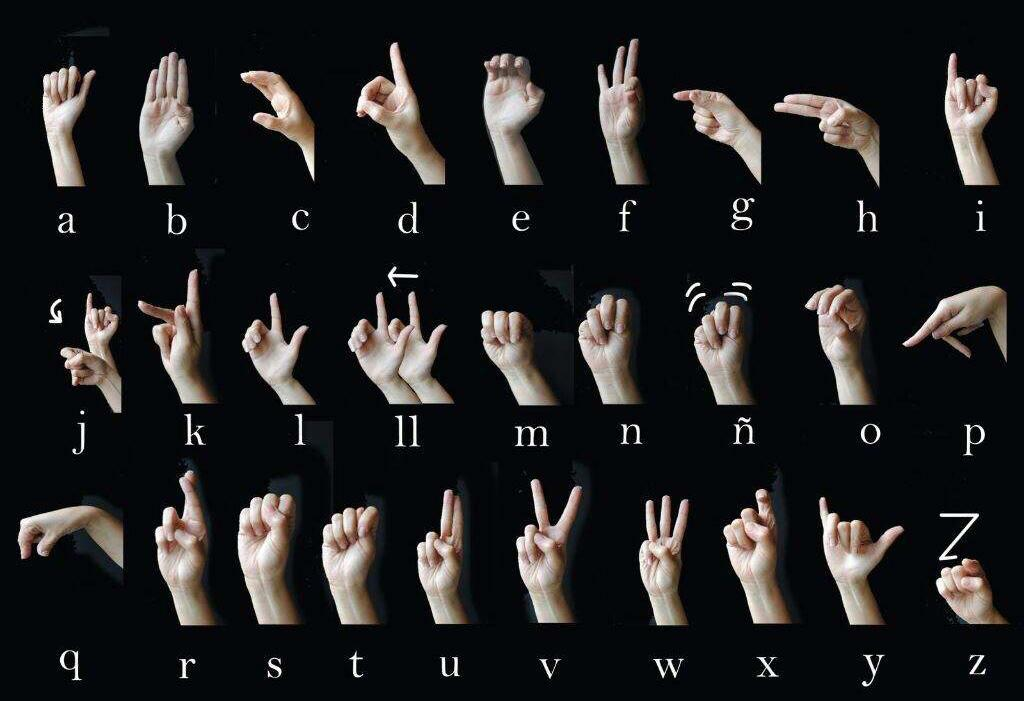
\includegraphics[width=14cm, height=10cm]{ABC.jpg}
	 \caption[Alfabeto internacional de señas]{Alfabeto internacional de señas\footnote{Matthew Chester, 2017,Amino, Lenguaje de Señas. "Abecedario de señas", Recuperado de: https://aminoapps.com/c/knka/page/blog/lenguaje-de-senas-abecedario-de-senas/BVPqG5swu57Vm}}%pie de la imagen
	 	 \label{fig:alfabeto}
\end{figure}

El alfabeto manual (de la fotografía) no es un lenguaje de señas, es solamente la representación de las letras del alfabeto atreves de distintas posiciones de las manos, por otro lado el lenguaje de señas tiene una estructura gramatical diferente de la del español, los signos tienen significado en sí mismos, como las palabras, pero ese significado puede ser alterado, enriquecido o  amplificado atreves de las expresiones faciales; un rostro sin expresión es tan aburrido como una voz monótona sin inflexiones y dice muy poco al receptor.

\subsection{Sistemas alternativos y aumentativos de comunicación (SAAC)}
\begin{itemize}
\item Sistemas aumentativos de comunicación: Son los que complementan el lenguaje oral, cuando por sí solo no es suficiente para entablar una comunicación efectiva con el entorno. El propósito de usar estos sistemas no es otro que el de apoyar y estimular la producción oral.
\item Sistemas alternativos de comunicación: Son los que sustituyen el lenguaje oral. Están dirigidos a aquellas personas que no tienen lenguaje oral, cuando no existen posibilidades de que el mismo se dé a corto o largo plazo.
\end{itemize}

Los sistemas alternativos y aumentativos de comunicación se clasifican dependiendo de si hacen uso de soportes o no, los cuales son:

\begin{itemize}
\item \textbf{Sistemas aumentativos y alternativos sin ayuda:} Estos sistemas se caracterizan por el hecho de que el emisor, para poder emitir mensajes compuestos por códigos no vocales/no orales, necesita un soporte físico externo a él. Sobre este soporte se incluyen diferentes elementos que se clasifican en función de su complejidad lingüística, de menor a mayor, en las siguientes categorías:
\begin{itemize}
\item Sistemas basados en elementos muy representativos: Estos elementos son objetos referenciales y están especialmente recomendados para personas con graves problemas de comunicación y representación.
\item Sistemas pictográficos: se utilizan fotografías, dibujos o símbolos.
\item Sistemas basados en la ortografía tradicional: los elementos de representación son el alfabeto escrito, es decir, letras, sílabas, palabras o frases. Evidentemente en estos casos las personas deben saber leer o escribir o estar en fase avanzada de adquisición de la lecto-escritura.
\end{itemize}

    \item \textbf{Sistemas aumentativos y alternativos sin ayuda:} Son mecanismos mediante los cuales las personas con alguna deficiencia o carencia lingüística pueden mejorar su comunicación sin hacer uso de apoyos externos. Se sirven del canal visual y utilizan la comunicación manual y/o gestual. Entre ellos se incluyen los siguientes sistemas: 
\begin{itemize}
\item Lenguaje de Signos: Es un sistema desarrollado de manera natural por la comunidad sorda. 
\item Sistema Bimodal: El Sistema Bimodal se deriva del Lenguaje de Signos. El mensaje se expresa en dos modalidades de forma simultánea: la signada y la hablada. La lengua base o dominante es la oral y es la que marca el orden de la frase y la que determina la sintaxis de las producciones. Es un sistema muy válido para la enseñanza de la lecto-escritura.
\item Dactilología: Se trata de una representación manual del alfabeto; cada letra tiene asignada una forma concreta de la mano.
\item Palabra Complementada: Es un sistema que hace posible percibir el habla a través de la vista mediante el uso simultáneo de la lectura labial y una serie limitada de complementos manuales. 
\item Mimo o Gesto Natural: El mimo y los gestos naturales se apoyan en herramientas comunes como son los movimientos, el cuerpo y las expresiones faciales y, contrariamente a los signos, son interpretados universalmente por todos los miembros de nuestra sociedad sin necesidad de un aprendizaje previo específico.\footnote{Centro de Documentación y Estudios, SIIS. (2012). Vivir mejor. Hacia una comunicación efectiva. Serie: Buenas Prácticas en la Atención a Personas con Discapacidad. Recuperado de: https://www.siis.net/}
\end{itemize}
\end{itemize}

\newpage
\subsection{Metodología SCRUM}
Un marco de trabajo por el cual las personas pueden acometer problemas complejos adaptativos, a la vez que entregar productos del máximo valor posible productiva y creativamente. 

Scrum es:

\begin{itemize}
\item Ligero 
\item Fácil de entender 
\item Extremadamente difícil de llegar a dominar.
\end{itemize}

Scrum es un marco de trabajo de procesos que ha sido usado para gestionar el desarrollo de productos complejos desde principios de los años 90. Scrum no es un proceso o una técnica para construir productos; en lugar de eso, es un marco de trabajo dentro del cual se pueden emplear varias técnicas y procesos. 

Scrum muestra la eficacia relativa de las prácticas de gestión de producto y las prácticas de desarrollo, de modo que podamos mejorar. 

El marco de trabajo Scrum consiste en los Equipos Scrum, roles, eventos, artefactos y reglas asociadas. Cada componente dentro del marco de trabajo sirve a un propósito específico y es esencial para el éxito de Scrum y para su uso.

Las reglas de Scrum relacionan los eventos, roles y artefactos, gobernando las relaciones e interacciones entre ellos. Las reglas de Scrum se describen en el presente documento.

Las estrategias específicas para usar el marco de trabajo Scrum son diversas y están descritas en otros lugares.

\textbf{ Teoría de Scrum }

Scrum se basa en la teoría de control de procesos empírica o empirismo. El empirismo asegura que el conocimiento procede de la experiencia y de tomar decisiones basándose en lo que se conoce. Scrum emplea un enfoque iterativo e incremental para optimizar la predictibilidad y el control del riesgo. 

Tres pilares soportan toda la implementación del control de procesos empírico: 

\begin{itemize}

\item \textbf{ Transparencia: }Los aspectos significativos del proceso deben ser visibles para aquellos que son responsables del resultado.

La transparencia requiere que dichos aspectos sean definidos por un estándar común, de tal modo que los observadores compartan un entendimiento común de lo que se está viendo.


\item \textbf{ Inspección:  }Los usuarios de Scrum deben inspeccionar frecuentemente los artefactos de Scrum y el progreso hacia un objetivo, para detectar variaciones. Su inspección no debe ser tan frecuente como para que interfiera en el trabajo. 

Las inspecciones son más beneficiosas cuando se realizan de forma diligente por inspectores expertos, en el mismo lugar de trabajo.


\item \textbf{ Adaptación: }Si un inspector determina que uno o más aspectos de un proceso se desvían de límites aceptables, y que el producto resultante no será aceptable, el proceso o el material que está siendo procesado deben ser ajustados. 

\end{itemize}
Dicho ajuste debe realizarse cuanto antes para minimizar desviaciones mayores. Scrum prescribe cuatro eventos formales, contenidos dentro del Sprint, para la inspección y adaptación, tal y como se describen en la sección Eventos de Scrum del presente documento. 

\begin{itemize}
\item Reunión de Planificación del Sprint (Sprint Planning Meeting) 
\item Scrum Diario (Daily Scrum) 
\item Revisión del Sprint (Sprint Review) 
\item Retrospectiva del Sprint (Sprint Retrospective) 
 
\end{itemize}
\textbf { El Equipo Scrum (Scrum Team) }

El Equipo Scrum consiste en un Dueño de Producto (Product Owner), el Equipo de Desarrollo (Development Team) y un Scrum Master. Los Equipos Scrum son autoorganizados y multifuncionales. Los equipos autoorganizados eligen la mejor forma de llevar a cabo su trabajo y no son dirigidos por personas externas al equipo.

\textbf {El Dueño de Producto (Product Owner) }

El Dueño de Producto es el responsable de maximizar el valor del producto y del trabajo del Equipo de Desarrollo. El cómo se lleva a cabo esto podría variar ampliamente entre distintas organizaciones, Equipos Scrum e individuos.

El Dueño de Producto es la única persona responsable de gestionar la Lista del Producto (Product Backlog). La gestión de la Lista del Producto incluye:
\begin{itemize} 
\item Expresar claramente los elementos de la Lista del Producto; 
\item Ordenar los elementos en la Lista del Producto para alcanzar los     objetivos y misiones de la mejor manera posible; 
\item Optimizar el valor del trabajo desempeñado por el Equipo de desarrollo; 
\item Asegurar que la Lista del Producto es visible, transparente y clara para todos, y que muestra aquello en lo que el equipo trabajará a continuación; y, 
\item Asegurar que el Equipo de Desarrollo entiende los elementos de la lista del Producto al nivel necesario. 
\end{itemize}

El Dueño de Producto podría hacer el trabajo anterior, o delegarlo en el Equipo de Desarrollo. Sin embargo, en ambos casos el Dueño de Producto sigue siendo el responsable de dicho trabajo.

\textbf{El Equipo de Desarrollo (Development Team) }

El Equipo de Desarrollo consiste en los profesionales que desempeñan el trabajo de entregar un Incremento de producto “Terminado”, que potencialmente se pueda poner en producción, al final de cada Sprint. Solo los miembros del Equipo de Desarrollo participan en la creación del Incremento.

Los Equipos de Desarrollo tienen las siguientes características: 
\begin{itemize}
\item Son auto organizados. Nadie (ni siquiera el Scrum Master) indica al Equipo de Desarrollo cómo convertir elementos de la Lista del Producto en Incrementos de funcionalidad potencialmente desplegables; 
\item Los Equipos de Desarrollo son multifuncionales, contando como equipo con todas las habilidades necesarias para crear un Incremento de producto; 
\item Scrum no reconoce títulos para los miembros de un Equipo de Desarrollo, todos son Desarrolladores, independientemente del trabajo que realice cada persona; no hay excepciones a esta regla; 
\item Scrum no reconoce sub-equipos en los equipos de desarrollo, no importan los dominios particulares que requieran ser tenidos en cuenta, como pruebas o análisis de negocio; no hay excepciones a esta regla; y, 
\item Los Miembros individuales del Equipo de Desarrollo pueden tener habilidades especializadas y áreas en las que estén más enfocados, pero la responsabilidad recae en el Equipo de desarrollo como un todo. 
\end{itemize}

\textbf {El Scrum Master }

El Scrum Master es el responsable de asegurar que Scrum es entendido y adoptado. Los Scrum Masters hacen esto asegurándose de que el Equipo Scrum trabaja ajustándose a la teoría, prácticas y reglas de Scrum. 

El Scrum Master es un líder que está al servicio del Equipo Scrum. El Scrum Master ayuda a las personas externas al Equipo Scrum a entender qué interacciones con el Equipo Scrum pueden ser de ayuda y cuáles no. El Scrum Master ayuda a todos a modificar estas interacciones para maximizar el valor creado por el Equipo Scrum.

\textbf {Eventos de Scrum} 

En Scrum existen eventos predefinidos con el fin de crear regularidad y minimizar la necesidad de reuniones no definidas en Scrum. Todos los eventos son bloques de tiempo (time-boxes), de tal modo que todos tienen una duración máxima. Una vez que comienza un Sprint, su duración es fija y no puede acortarse o alargarse.
 Los demás eventos pueden terminar siempre que se alcance el objetivo del evento, asegurando que se emplee una cantidad apropiada de tiempo sin permitir desperdicio en el proceso.
 
\textbf {El Sprint }

El corazón de Scrum es el Sprint, es un bloque de tiempo (time-box) de un mes o menos durante el cual se crea un incremento de producto “Terminado”, utilizable y potencialmente desplegable.
Es más conveniente si la duración de los Sprints es consistente a lo largo del esfuerzo de desarrollo. Cada nuevo Sprint comienza inmediatamente después de la finalización del Sprint previo. 

Los Sprints contienen y consisten de la Reunión de Planificación del Sprint (Sprint Planning Meeting), los Scrums Diarios (Daily Scrums), el trabajo de desarrollo, la Revisión del Sprint (Sprint Review), y la Retrospectiva del Sprint (Sprint Retrospective).

Durante el Sprint: 
\begin{itemize}
\item No se realizan cambios que puedan afectar al Objetivo del Sprint (Sprint Goal); 
\item Los objetivos de calidad no disminuyen; y, 
\item El alcance puede ser clarificado y renegociado entre el Dueño de Producto y el Equipo de Desarrollo a medida que se va aprendiendo más. 
\end{itemize}

Cada Sprint puede considerarse un proyecto con un horizonte no mayor de un mes. Al igual que los proyectos, los Sprints se usan para lograr algo. 

Cada Sprint tiene una definición de qué se va a construir, un diseño y un plan flexible que guiará la construcción y el trabajo y el producto resultante.

Los Sprints están limitados a un mes calendario. Cuando el horizonte de un Sprint es demasiado grande la definición de lo que se está construyendo podría cambiar, la complejidad podría elevarse y el riesgo podría aumentar. 

Los Sprints habilitan la predictibilidad al asegurar la inspección y adaptación del progreso al menos en cada mes calendario. Los Sprints también limitan el riesgo al costo de un mes calendario.

\textbf { Cancelación de un Sprint } 

Un Sprint puede ser cancelado antes de que el bloque de tiempo llegue a su fin. Solo el Dueño de Producto tiene la autoridad para cancelar el Sprint, aunque puede hacerlo bajo la influencia de los interesados, del Equipo de Desarrollo o del Scrum Master. 

Un Sprint se cancelaría si el Objetivo del Sprint llega a quedar obsoleto. Esto podría ocurrir si la compañía cambia la dirección o si las condiciones del mercado o de la tecnología cambian. 

En general, un Sprint debería cancelarse si no tuviese sentido seguir con él dadas las circunstancias. Pero debido a la corta duración de los Sprints, rara vez la cancelación tiene sentido. 

Cuando se cancela un Sprint, se revisan todos los Elementos de la Lista de Producto que se hayan completado y “Terminado”. Si una parte del trabajo es potencialmente entregable, el Dueño de Producto normalmente lo acepta. Todos los Elementos de la Lista de Producto no completados se vuelven a estimar y se vuelven a introducir en la Lista de Producto. El trabajo finalizado en ellos pierde valor con rapidez y frecuentemente debe volverse a estimar. 

Las cancelaciones de Sprint consumen recursos, ya que todos deben reagruparse en otra Reunión de Planificación de Sprint para empezar otro Sprint. Las cancelaciones de Sprint son a menudo traumáticas para el Equipo Scrum y son muy poco comunes.\footnote{Schwaber K. Sutherland J. (2013). La Guia de Scrum. Recuperado de https://www.scrumguides.org}


\newpage

\section{Herramientas para el Desarrollo del Software}
\subsection{Herramientas de Software}
\subsection{Lenguaje de programación}
\textbf{Python}

Python es un lenguaje de programación interpretado de tipado dinámico cuya filosofía hace hincapié en una sintaxis que favorezca un código legible. Se trata de un lenguaje de programación multiparadigma y disponible en varias plataformas.\footnote{Miguel Ángel Abellán. (2019). Curso de iniciación a Python en Raspberry Pi. Murcia, España. Programo Ergo Sum.
https://www.programoergosum.com/cursos-online/raspberry-pi/244-iniciacion-a-python-en-raspberry-pi/que-es-python}

   \textbf{Características de Python}
   
Es un lenguaje interpretado , esto quiere decir que se ejecuta en tiempo real en cualquier plataforma que tenga un intérprete, es una gran ventaja cuando queremos hacer pequeñas modificaciones en una aplicación y no tenemos que recompilar toda cada vez que hagamos un cambio, lo cual nos permite ser más eficaces a la hora de programar .

El único aspecto negativo de los interpretados es ser interpretado es que son menos eficientes a la hora de ser interpretados. Como no es compilada, Python debe ser traducido a código máquina con cada ejecución, esto hace que tanto Python como otros interpretados sean más lentos en la ejecución.

Es un lenguaje de alto nivel , esto quiere decir que está hecho para que los humanos lo entendamos sin dificultad alguna . Otra gran ventaja, es que si queremos, podemos trabajar con bits y bytes en Python como si fuera de medio nivel.

Es multiparadigma, podremos crear más de un programa con más de un estilo de desarrollo diferente. nos permite usar programación modular, estructurada, orientada a objetos entre otros dependiendo de lo que sea más eficiente para crear nuestro programa.

Es libre , por tanto tenemos el código fuente disponible para conocerlo y estudiarlo a fondo. Además, tiene una gran comunidad detrás para cualquier tipo de ayuda que necesitemos, aparte de una documentación realmente buena disponible gratuitamente.

   \textbf{Ventajas de Python}
   
Python es fácil de aprender . Su curva de aprendizaje es bastante adecuada, con la combinación apropiada de motivación y atención podrás crear un programa sin conocimientos previos.\footnote{Domingo Muñoz, J. 2017. España. OpenWebinars. https://openwebinars.net/blog/por-que-aprender-a-programar-python/}

   \textbf{Licencia de uso}
   
Python se desarrolla bajo una licencia de Open source o código abierto aprobada por OSI, por lo que se puede usar y distribuir libremente, incluso para uso comercial.
La licencia de Python es administrada por Python Software Foundation.
\begin{figure}[H]
\centering
	 
\includegraphics[width=7cm, height=7cm]{Open_Source.png}
	 \caption[Logotipo de la Open Source Initiative]{Logotipo de la Open Source Initiative\footnote{Domingo Muñoz, J. 2017. España. OpenWebinars. https://openwebinars.net/blog/por-que-aprender-a-programar-python/}}%pie de la imagen
	 	 \label{fig:Open Source Initiative}
\end{figure}

   \textbf{Python Software Foundation}
   
La Python Software Foundation (PSF) es una corporación sin fines de lucro 501 (c) (3) que posee los derechos de propiedad intelectual detrás del lenguaje de programación Python. Administran las licencias de código abierto para Python versión 2.1 y posteriores, y poseen y protegen las marcas comerciales asociadas con Python.
También, realizan la conferencia PyCon de Norteamérica anualmente, apoyan otras conferencias de Python en todo el mundo y financia el desarrollo relacionado con Python con nuestro programa de subvenciones y financia proyectos especiales.\footnote{Covantec R.L.(2014 - 2018). Acerca de Python. Introducción al lenguaje Python. Recuperado de: https://entrenamiento-python-basico.readthedocs.io/es/latest/leccion1/introduccion.html.}\\

\subsection{Entornos de desarrollo}
\textbf {PyCharm}

PyCharm es uno de los entornos de desarrollo más completos para Python. Es parte del suite de herramientas de programación ofrecidas por JetBrains, que cuenta con entornos para construir código en distintos idiomas como PHP.

\textbf {Ventajas de PyCharm}

Trabajar con PyCharm tiene ventajas básicas (similares a las ofrecidas por otros IDE) pero también algunas específicas a las cuales debe su popularidad. Es así que PyCharm tiene un editor inteligente, que permite completar código con algunos atajos de teclado. Asimismo, permite navegar a través de nuestro código, saltando entre las clases y métodos creados, haciendo el flujo de trabajo mucho más dinámico.

Una de las características notables de PyCharm es la posibilidad que tiene de refactorizar el código, que, en términos generales, significa modificar el código sin comprometer la ejecución del mismo.
Esta operación se realiza de forma constante dentro de la Ingeniería de Software y es más conocida como limpiar el código para que este pueda ser interpretado con facilidad cuando hay distintas personas integrando un equipo de trabajo.

Por último, la gran cantidad de desarrolladores que trabajan con PyCharm ha generado que se tenga una gran cantidad de temas y plugins que se pueden usar para trabajar más cómodamente.

Ellos permiten la integración con otros lenguajes y frameworks (como Node JS) y un acceso más fácil a bases de datos y debugging.\footnote{Escuela de Python. (2019). PyCharm: uno de los mejores IDE para Python. Recuperado de: https://www.escuelapython.com/pycharm-uno-de-los-mejores-ide-para-python.}\\


\textbf{Software Arduino}

El software de Arduino es un IDE, entorno de desarrollo integrado (siglas en inglés de Integrated Development Environment). Es un programa informático compuesto por un conjunto de herramientas de programación. El IDE de Arduino es un entorno de programación que ha sido empaquetado como un programa de aplicación; es decir, consiste en un editor de código, un compilador, un depurador y un constructor de interfaz gráfica (GUI). Además, incorpora las herramientas para cargar el programa ya compilado en la memoria flash del hardware. \footnote{Enrique Crespo. (2016). Entorno de Programación Arduino (IDE). Zaragoza, España. Aprendiendo Arduino. https://aprendiendoarduino.wordpress.com/2016/03/29/entorno-de-programacion-de-arduino-ide.}
El software de código abierto Arduino (IDE) facilita escribir código y cargarlo en la pizarra. Se ejecuta en Windows, Mac OS X y Linux. El entorno está escrito en Java y se basa en Procesamiento y otro software de código abierto. 

\subsection{Sistema de Base de Datos}
\textbf{María DB}

MariaDB es un sistema de base de datos que proviene de MySQL, pero con licencia GPL, desarrollado por Michael Widenius, fundador de MySQL y la comunidad de desarrolladores de software libre. \footnote{Drauta,  G. A. (2016). https://www.drauta.com/que-es-mariadb}

\textbf{Ventajas de Maria DB:}
\begin{itemize}
\item Incorpora nuevos motores de almacenamiento mucho más eficientes que son Aria y XtraDB, los cuales han sido desarrollados para ser los sustitutos de MyISAM e InnoDB respectivamente. Estos permiten ejecutar consultas más complejas y almacenarlas en caché y no en disco duro.
\item Aparte de incluir los sustitutos de MyISAM e InnoDB también incorpora nuevos motores de almacenamiento.
\item También incorpora mejoras de rendimiento y versiones de seguridad más rápidas y más transparentes.
\item Es de código libre y cuenta con el soporte de la comunidad de desarrolladores, pero también cuenta con el soporte de Oracle.
\end{itemize}


\subsection{Herramientas de Hardware}

\textbf{Arduino UNO}

Arduino es una plataforma de hardware libre, basada en una placa con un microcontrolador y un entorno de desarrollo, diseñada para facilitar el uso de la electrónica en proyectos multidisciplinares. Por otro lado, Arduino nos proporciona un software consistente en un entorno de desarrollo (IDE) que implementa el lenguaje de programación de arduino y el bootloader ejecutado en la placa. La principal característica del software de programación y del lenguaje de programación es su sencillez y facilidad de uso. Arduino se puede utilizar para desarrollar elementos autónomos, conectándose a dispositivos e interactuar tanto con el hardware como con el software.

Es una placa basada en el microcontrolador ATmega328P. Tiene 14 pines de entrada/salida digital (de los cuales 6 pueden ser usando con PWM), 6 entradas analógicas, un cristal de 16Mhz, conexión USB, conector jack de alimentación, terminales para conexión ICSP y un botón de reseteo. Tiene toda la electrónica necesaria para que el microcontrolador opere, simplemente hay que conectarlo a la energía por el puerto USB ó con un transformador AC-DC.

\begin{figure}[H]
\centering
	 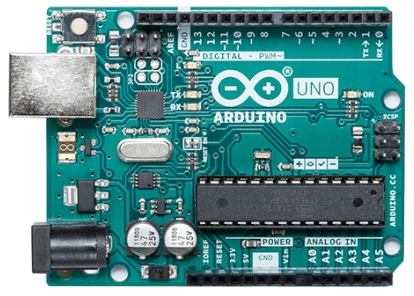
\includegraphics[width=10cm, height=7cm]{Arduino1.png}
	 \caption[Placa Arduino UNO]{Placa Arduino UNO}
	 	 \label{fig:arduino}
\end{figure}

%Ref. http://alsw.net/tienda/arduino/arduino_original/arduinogenino-mega2560-r3/ 


\textbf{Licencias de Uso}

Arduino es una plataforma de hardware libre, basada en una placa con un microcontrolador y un entorno de desarrollo, diseñada para facilitar el uso de la electrónica en proyectos multidisciplinares. 

El hardware consiste en una placa con un microcontrolador Atmel AVR y puertos de entrada/salida. Los microcontroladores más usados son el Atmega168, Atmega328, Atmega1280, ATmega8 por su sencillez y bajo coste que permiten el desarrollo de múltiples diseños. Por otro lado, el software consiste en un entorno de desarrollo que implementa el lenguaje de programación Processing/Wiring y el cargador de arranque (boot loader) que corre en la placa. Arduino se puede utilizar para desarrollar objetos interactivos autónomos o puede ser conectado a software del ordenador (por ejemplo: Macromedia Flash, Processing, Max/MSP, Pure Data). El entorno de desarrollo integrado libre se puede descargar gratuitamente. 

Al ser open-hardware, tanto su diseño como su distribución es libre. Es decir, puede utilizarse libremente para el desarrollo de cualquier tipo de proyecto sin haber adquirido ninguna licencia. 
Las placas pueden ser hechas a mano o compradas montadas de fábrica; el software puede ser descargado de forma gratuita. Los ficheros de diseño de referencia (CAD) están disponibles bajo una licencia abierta, así pues, eres libre de adaptarlos a tus necesidades.\\
\textbf{Características técnicas:}\\

\begin{table}[htbp]
\begin{tabular}{|c|c|}
\hline
\textbf{Microcontrolador}                 & ATmega328P                                                                                                             \\ \hline
\textbf{ATmega328P}                       & 5V                                                                                                                     \\ \hline
\textbf{Voltaje de entrada (recomendado)} & 7-12V                                                                                                                  \\ \hline
\textbf{Voltaje de entrada (límite)}      & 6-20V                                                                                                                  \\ \hline
\textbf{Digital pines I/O}                & 14 (de los cuales 6 proporcionan una salida PWM)                                                                       \\ \hline
\textbf{PWM digital pines I/O}            & 6                                                                                                                      \\ \hline
\textbf{Pines de entrada analógica}       & 6                                                                                                                      \\ \hline
\textbf{Corriente DC por Pin I/O}         & 24mA                                                                                                                   \\ \hline
\textbf{Corriente DC para Pin 3.3V}       & 60mA                                                                                                                   \\ \hline
\textbf{Memoria flash}                    & \begin{tabular}[c]{@{}c@{}}32KB ATmega328P de los que 0,5 KB son utilizados por \\el gestor de arranque.\end{tabular} \\ \hline
\textbf{SRAM}                             & 2KB ATmega328P                                                                                                         \\ \hline
\textbf{EEPROM}                           & 1KB ATmega328P                                                                                                         \\ \hline
\textbf{Velocidad de reloj}               & 16 MHZ                                                                                                                 \\ \hline
\textbf{Longitud}                         & 68,6 mm                                                                                                                \\ \hline
\textbf{Anchura}                          & 53,4 mm                                                                                                                \\ \hline
\textbf{Peso}                             & 25 g                                                                                                                   \\ \hline
\end{tabular}
\caption{Características técnicas}

\end{table}

\textbf{Descripción de los pines de Arduino Uno}\footnote{Infootec.net. Arduino Uno R3 .Recuperado de: https://www.infootec.net/arduino/}

\begin{itemize}
\item\textbf{Pin VIN:} 
Este pin se puede usar de varias formas, si tenemos una fuente de alimentación conectada mediante un adaptador, lo que podemos hacer mediante este pin es obtener la alimentación para conectar otro dispositivo pero tenemos que tener en cuenta que la placa no regulara la tensión y obtendremos la misma tensión que tenga el adaptador. Por otro lado si tenemos conectado el USB, la tensión será regulada a 5v. Y si tenemos una fuente de alimentación externa como por ejemplo pilas, el borne positivo de la pila ira conectado al pin VIN y el borne negativo de la pila al pin GND, en este caso si la pila saca 10v la placa regulara la tensión a 5v.
\item\textbf{Pin GND:} El pin GND es la tierra.
\item \textbf{Pin 5v:} Este pin tiene varias funciones, podemos alimentar la placa mediante este pin, siempre que tengamos la fuente externa regulada a 5v. Por otro lado si tenemos la placa alimentada tanto por el Jack como por USB, se puede alimentar otro componente con una tensión regulada de 5v.
\item \textbf{Pin 3.3v:} Por este pin sacamos una tensión de 3.3v que es alimentada mediante el conector Jack o el USB. Los 3.3v se utilizan para alimentar dispositivos que requieren una tensión baja.
\end{itemize}

\textbf{Pines de entradas analógicas}

La placa de Arduino cuenta con 6 pines de entradas analógicas, que van desde el pin A0 al A5, de los cuales proporcionan 10bits, llamados bits de resolución. La tensión que miden va de 0 a 5v, aunque es posible cambiar su rango usando una función con el pin AREF.

\begin{itemize}
\item \textbf{Pin IOREF:} El pin IOREF es una copia del pin VIN y se utiliza para indicar a los demás dispositivos conectador a la placa que las tensiones de los pines de entrada y salida son 5v.
\item \textbf{Pin RESET:} Este pin tiene el mismo funcionamiento que el botón RESET, se utiliza para reiniciar el microcontrolador.
\item \textbf{Pines de entradas y salidas digitales:} Las entradas y salidas digitales son 14 y van desde el pin 0 al 13 y ofrecen una tensión de 5v
\item \textbf{Pines  A5 SCL y A4 SDA:} Se pueden utilizar para conectar dispositivos que lleven a cabo comunicaciones mediante la librería Wire.
\item \textbf{Pin AREF:} Ofrece un voltaje de referencia para las entradas analógicas.
\item \textbf{Pines 1 TX y 0 RX:} Estos pines se utilizan para recibir y transmitir datos en serie.
\end{itemize}

\begin{figure}[H]
\centering
	 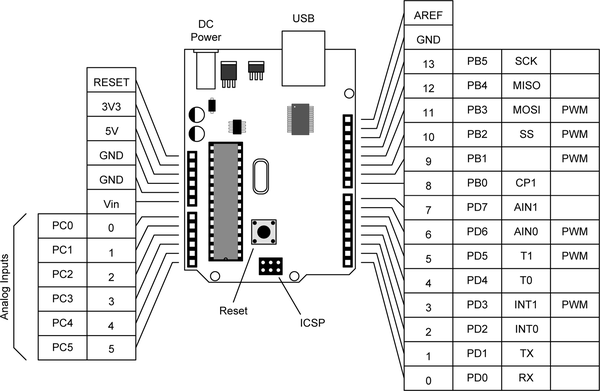
\includegraphics[width=10cm, height=7cm]{Arduino1pines.png}
	 \caption{Diagrama de pines Arduino UNO}%pie de la imagen
	 	 \label{fig:Arduinopines}
\end{figure}

\textbf{Sensores flexores 2.2}\\
Un simple sensor flexible de 2.2 pulgadas de longitud. A medida que el sensor se flexiona, la resistencia aumenta a través del sensor.	
La resistencia del sensor de flexión cambia cuando las almohadillas de metal están en el exterior de la curva (el texto está dentro de la curva). \footnote{ Symbol. (2014) Flex Sensor. Utah, EU.: Spectra Symbol.Recuperado de: https://www.spectrasymbol.com/wp-content/uploads/2016/12/FLEX-SENSOR-DATA SHEET-v2014-Rev-A.}
%Ref “”https://www.sparkfun.com/products/10264””

\begin{figure}[h!]
\centering
	 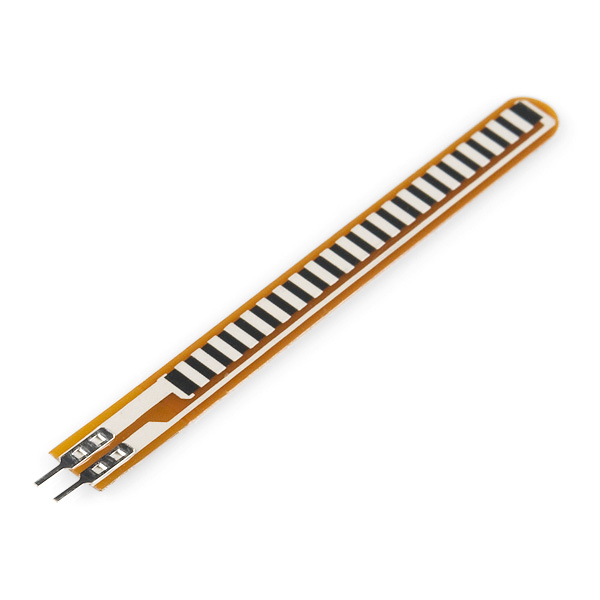
\includegraphics[width=10cm, height=7cm]{sensorf.jpg}
	 \caption[Sensor Flex 2.2]{Sensor Flex 2.2}%pie de la imagen
	 	 \label{fig:sensorFlex}
\end{figure}

\textbf{Descripción:}

El sensor de flexión de 2.2 varía su resistencia al ser doblado. Puedes utilizar este sensor en conjunto de un divisor de tensión para obtener un valor analógico de 0 a 5V en su salida. Este producto corresponde a una tecnología patentada de Spectra Symbol.

La resistencia del sensor flex cambia cuando los pads metálicos se encuentran en el interior del doblez. Este sensor posee 30Kohm en un estado normal de reposo (sin flexión) y cuando esta doblado en un ángulo de 90 grados su resistencia aumenta hasta 70Kohm.

\textbf{Características:}
\begin{itemize}
\item Medición de desplazamiento de ángulo.
\item Dobla y flexiona físicamente con dispositivo de movimiento.
\item Posibles usos: robótica, Juegos (movimiento virtual), Dispositivos médicos, Periféricos de la computadora.
\item Construcción simple.
\item Perfil bajo.
\end{itemize}

\textbf{Uso de Flex Sensor con Arduino}

El sensor tiene en sí varios sensores que cambian en la resistencia en función de la cantidad de curvatura que se le emplea, convierten el cambio en la curva a la resistencia eléctrica a mayor sea la curva, mayor será el valor de la resistencia. Se emplean en los guantes para detectar el movimiento del dedo, para controlar automóviles, productos de fitness, aparatos de medición , tecnología de asistencia, instrumentos musicales, smartphones, entre otros.

Su principal desarrolló inicial fue para las bolsas de aire para los carros, hoy en día se usa hasta en bocinas de los carros, juguetes que detectan diferentes grados de presión o de flexión entre otros.\footnote{Gusin S., 2012, Uso de Flex Sensor con Arduino, computointegrado, recuperado de: http://computointegrado.blogspot.com/2012/04/uso-de-flex-sensor-con-arduino.html}   

Ahora veamos los pines del flex sensor:
\newpage
\begin{figure}[H]
\centering
	 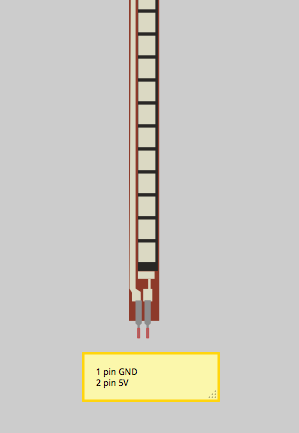
\includegraphics[width=10cm, height=7cm]{pines-sensor.png}
	 \caption[Pines Sensor Flex 2.2]{Pines Sensor Flex 2.2  }%pie de la imagen
	 	 \label{fig:PinessensorFlex}
\end{figure}
Además del flex sensor necesitaremos una resistencia de 47K ohms, una vez obtenido el material pasaremos al circuito.
\begin{figure}[H]
\centering
	 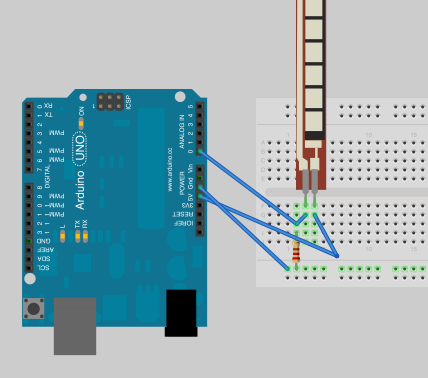
\includegraphics[width=10cm, height=7cm]{diagrama-de-sensor.png}
	 \caption[Diagrama Sensor Flex 2.2 a Arduino]{Diagrama Sensor Flex 2.2 a Arduino   }%pie de la imagen
	 	 \label{fig:DiagramasensorFlex}
\end{figure}

\newpage
\textbf{Resistencia 47K ohms}

Las resistencias o resistores son los elementos mas utilizados en electrónica y son utilizados en infinidad de proyectos, ya sea para limitar la corriente por ejemplo en un LED , como divisor de voltaje,  para disipar potencia como en el caso de los arreglos de resistencia para motores eléctricos,  o también para generar calor como las resistencias eléctricas que utilizan las cafeteras, calentadores de agua, etc.

La resistencia de 47 K ohms a 1/4 de watt con una tolerancia del 5 por ciento  resiste un voltaje máximo de 300V , gracias a su forma pueden ser fácilmente incorporadas tanto a un protoboard como a una tablilla perforada o ser soldada directamente. \footnote{Nextia Fenix, Resistencia 47K ohms @ 1/4W, https://www.nextiafenix.com/producto/resistencia-47k-1w4/}   

\begin{figure}[H]
\centering
	 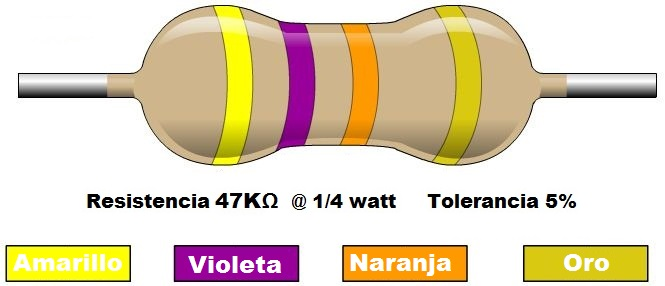
\includegraphics[width=10cm, height=7cm]{resistencia.jpg}
	 \caption[Resistencia 47K ohms]{Resistencia 47K ohms}%pie de la imagen
	 	 \label{fig:Resistencia47K}
\end{figure}

    \textbf{Breadboard}
    
 Un breadboard (protoboard) es un dispositivo para prototipado temporal sin soldadura con componentes electrónicos y probar diseño de circuitos. La mayoría de los componentes electrónicos en circuitos electrónicos pueden ser interconectados insertando sus conexiones o terminales en los huecos y luego haciendo conexiones a través de cables donde es apropiado. El breadboard tiene líneas metálicas que están establecidas como se muestra más abajo. Note que las líneas de puntos de arriba y de abajo están conectadas horizontalmente y divididas en la mitad mientras que el resto de los huecos están conectados verticalmente.\footnote{B. Hernando, Wiring, Qué es un breadboard o protoboard?, http://wiring.org.co/learning/tutorials/es/breadboard/index.html.}   
    
 \begin{figure}[H]
\centering
	 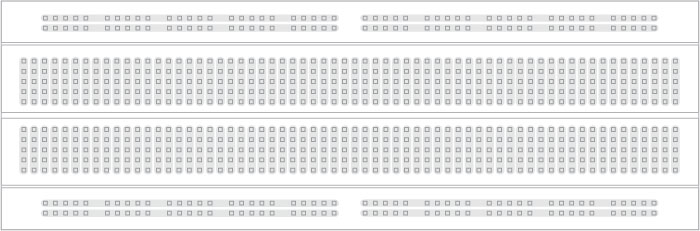
\includegraphics[width=10cm, height=7cm]{breadboard-01.jpg}
	 \caption[Breadboard]{Breadboard  }%pie de la imagen
	 	 \label{fig:Breadboard}
\end{figure}
 
 \textbf{Jumper}
 
Son pequeños cables removibles para realizar conexiones, sin soldaduras, sin falsos contactos y sin desorden para protoboard. Los cables vienen cada uno con su conector independiente. Evita que los cables que se rompen y se atoren en el protoboard.
Estos cables son ideales para realizar las primeras prácticas con Arduino y microcontroladores, sin embargo, para circuitos complejos pueden no ser tan convenientes, son ideales para realizar montajes temporales en el protoboard. \footnote{Geek Factory,Jumpers para protoboard 65 cables , https://www.geekfactory.mx/tienda/cables-y-conectores/jumpers-para-protoboard-65-cables/.}   
\newpage
 \begin{figure}[H]
\centering
	 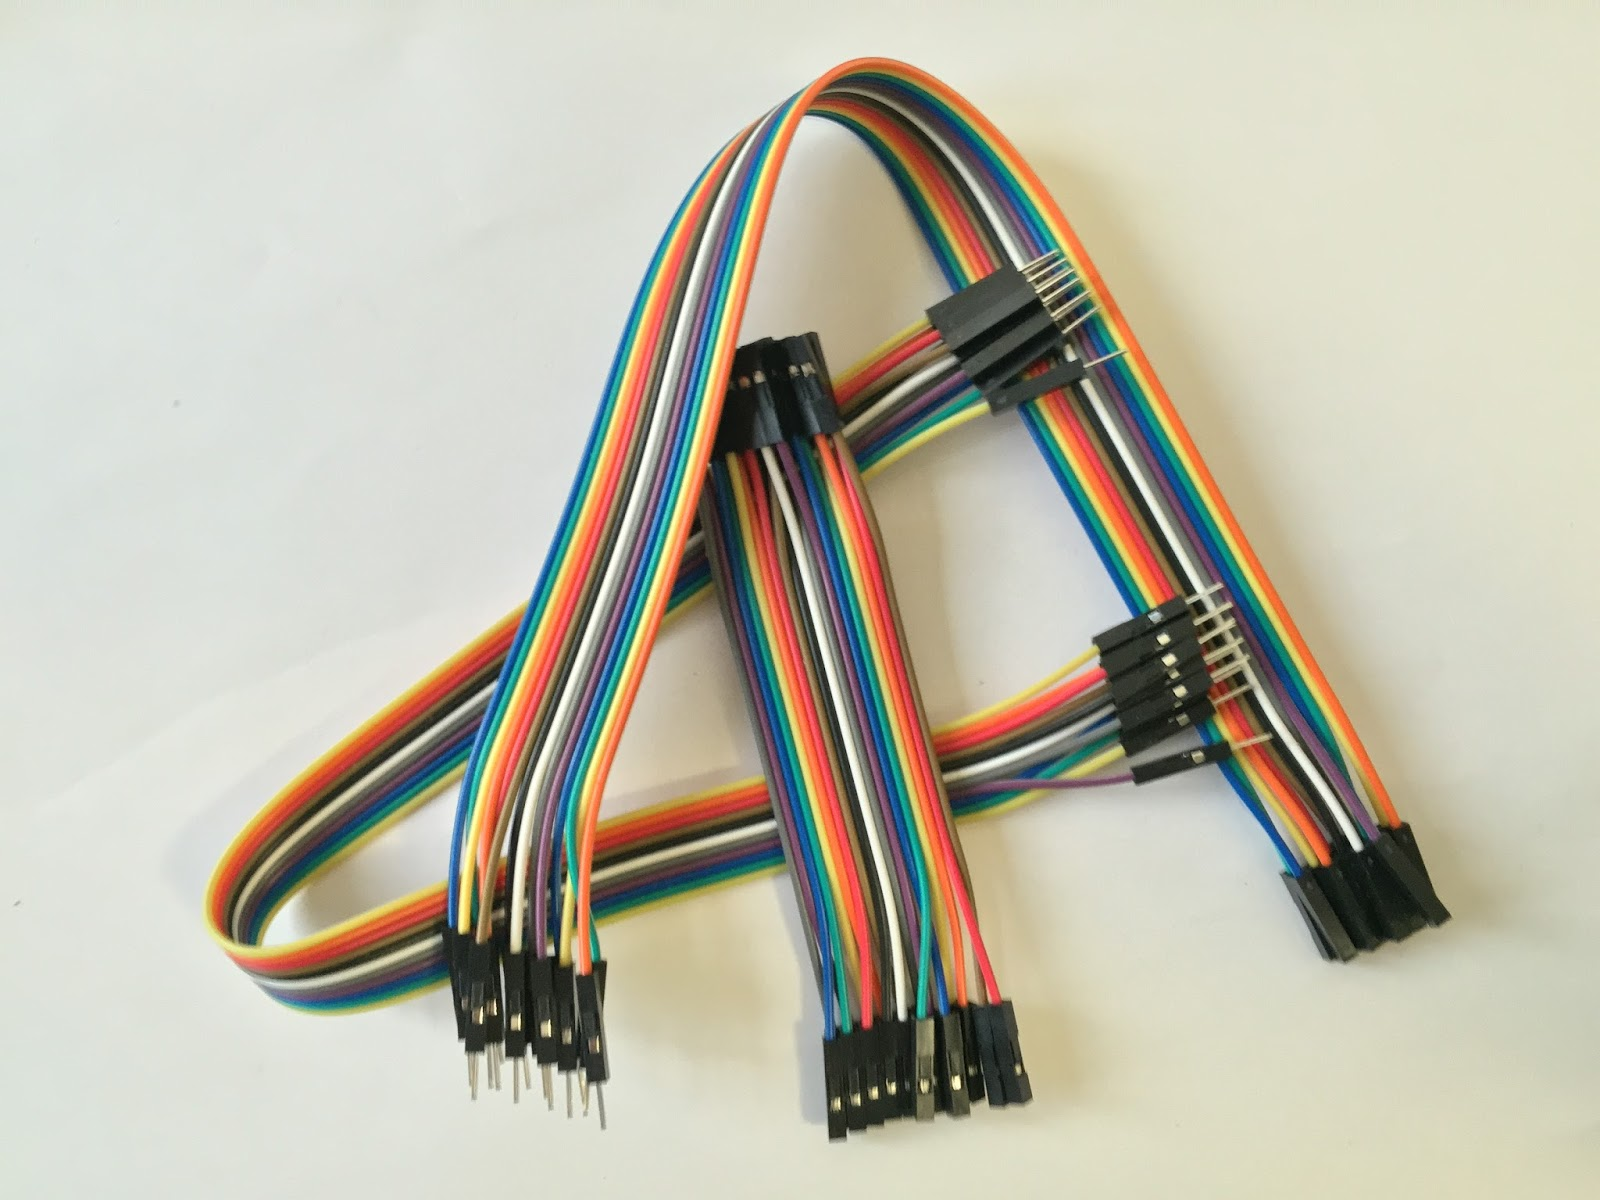
\includegraphics[width=10cm, height=7cm]{Jumpers.JPG}
	 \caption[Jumpers]{Jumpers}%pie de la imagen
	 	 \label{fig:Jumpers}
\end{figure}




\section{Marco Legal}
\subsection{Ley de propiedad intelectual}
La propiedad intelectual hace referencia a los derechos exclusivos otorgados por el Estado sobre las creaciones del intelecto humano, en particular, las invenciones, las obras literarias y artísticas, y los signos y diseños distintivos utilizados en el comercio.\footnote{Organización Mundial de la Propiedad Intelectual. (2016). ¿Qué son los derechos de propiedad intelectual? ¿De qué manera están al servicio de las Pymes del sector farmacéutico? New York, Estados Unidos. Recuperado de https://www.wipo.int/sme/es/documents/ippharma.html}

Según el Art. 1. Las disposiciones contenidas en la presente ley tienen por objeto asegurar una protección suficiente y efectiva de la propiedad intelectual, estableciendo las bases que la promuevan, fomenten y protejan.

Esta ley comprende el derecho de autor, los derechos conexos y la propiedad industrial en lo relativo a invenciones, modelos de utilidad, diseños industriales y secretos industriales o comerciales y datos de prueba.

En el reglamento de la Administración Académica de la Universidad de El Salvador según Art. 215 se estipula que los derechos de autor sobre los trabajos de investigación elaborados en los procesos de graduación serán de propiedad exclusiva de la Universidad, la cual podrá disponer de los mismos de conformidad a su marco jurídico interno y legislación aplicable.

Por lo tanto, los derechos de autor del proyecto informático producto de la investigación son exclusivos de la Universidad de El Salvador.


\subsection{Licencia de Software}
\subsubsection{Copyleft}
El copyleft es un método general para liberar un programa u otro tipo de trabajo (en el sentido de libertad, no de gratuidad), que requiere que todas las versiones modificadas y extendidas sean también libres.

La manera más simple de hacer que un programa sea software libre consiste en ponerlo en el dominio público, sin copyright. 

Esto permite compartir el programa y sus mejoras a quienes así lo deseen. Sin embargo, también posibilita que otra gente sin interés cooperativo convierta el programa en software privativo. Pueden hacer cambios, muchos o pocos, y distribuir el resultado como un producto privativo. Quienes reciban el programa modificado en esas condiciones no podrán disfrutar de la libertad que el autor original les dio.\footnote{Free Software Foundation, Inc.(2018). ¿Qué es el Copyleft? Boston, Massachusetts, Estados Unidos. Recuperado de https://www.gnu.org/licenses/copyleft.es.html}


\subsection{Código Fuente}
\subsubsection{Licencia Pública General}

La Licencia Pública General de GNU, llamada comúnmente GPL de GNU, se usa para la mayoría de los programas de GNU y para más de la mitad de los paquetes de software libre. La última es la versión 3. 

Es una licencia de software libre copyleft publicada por la Free Software Foundation. Los usuarios de un programa con licencia GPL son libres para usarlo, acceder al código fuente, modificarlo y distribuir los cambios; siempre que redistribuyan el programa completo (modificado o no modificado) bajo la misma licencia. \footnote{GNU. (2018). Licencias. Recuperado de: https://www.gnu.org/licenses/licenses.es.html }

\subsection{Licencia de derechos autorales}
\subsubsection{Licencia Creative Commons}

Las licencias y herramientas de derechos autorales Creative Commons, forja un equilibrio dentro del escenario tradicional de «todos los derechos reservados» que crean las leyes de derechos autorales.

Las imágenes, vídeos y sonido, estarán bajo la licencia Creative Commons Atribución-NoComercial-SinDerivadas (CC BY-NC-ND).

\textbf{Atribución-NoComercial-SinDerivadas (CC BY-NC-ND)}

Esta licencia solo permite compartir, es decir,  copiar y redistribuir el material en cualquier medio o formato.

Bajo los siguientes términos:
\begin{itemize}
\item Atribución — Debe dar crédito de manera adecuada, brindar un enlace a la licencia, e indicar si se han realizado cambios. Puede hacerlo en cualquier forma razonable, pero no de forma tal que sugiera que usted o su uso tienen el apoyo de la licenciante.

\item NoComercial — No puede hacer uso del material con propósitos comerciales.

\item SinDerivadas — Si remezcla, transforma o crea a partir del material, no podrá distribuir el material modificado. \footnote{Creative Commons. (2016). Atribución-NoComercial-SinDerivadas 4.0 Internacional. Recuperado de:  https://creativecommons.org/licenses/by-nc-nd/4.0/deed.es}
\end{itemize}
\newpage
\section{Marco Conceptual}
\begin{itemize}


\item \textbf{Alfabetización:} concibe como un proceso gradual de aprendizaje que posibilita la comprensión de la lectura, la expresión escrita y el uso del cálculo matemático básico.

\item \textbf{ASL:} Lenguaje de Signos Americano.

\item \textbf{CONAIPD:} Consejo Nacional de Atención Integral a la Persona con discapacidad.

\item \textbf{Dactilología:} Se trata de una representación manual del alfabeto; cada letra tiene asignada una forma concreta de la mano.

\item \textbf{Défecit: } es aquella situación que se genera cuando hay escasez de algo necesario.

\item \textbf{Discapacidad auditiva: }Es un déficit total o parcial en la percepción que se evalúa por el grado de pérdida de la audición en cada oído.
\item \textbf{Discriminación: }fenómeno sociológico en los seres humanos que atenta contra la igualdad.

\item \textbf{Educación inclusiva: }proceso de identificar y responder a la diversidad de las necesidades de todos los estudiantes a través de la mayor participación en el aprendizaje, las culturas y las comunidades, y reduciendo la exclusión en la educación.

\item \textbf{Hardware:} conjunto de los componentes que conforman la parte material (física) de una computadora, a diferencia del software que refiere a los componentes lógicos (intangibles).

\item \textbf{Hipoacúsico: }Persona con pérdida o discapacidad auditiva.

\item \textbf{Lectoescritura: }capacidad y habilidad de leer y escribir adecuadamente, pero también, la lectoescritura constituye un proceso de aprendizaje en el cual los educadores pondrán especial énfasis durante la educación inicial proponiendo a los niños diversas tareas que implican actividades de lectoescritura.

\item \textbf{Lengua de señas: }es un lenguaje natural de expresión y configuración gesto-espacial y percepción visual, gracias a la cual, las personas con discapacidad auditiva pueden establecer un canal de comunicación con su entorno social, ya sea conformado por otros individuos sordos o por cualquier persona que conozca la lengua de señas empleada.

\item \textbf{LESSA:} Lengua de Señas Salvadoreña.

\item \textbf{Léxico: }es el vocabulario de un idioma o de una región, el diccionario de una lengua o el caudal de modismos y voces de un autor.

\item \textbf{Metodología: }serie de métodos y técnicas de rigor científico que se aplican sistemáticamente durante un proceso de investigación para alcanzar un resultado teóricamente válido. En este sentido, la metodología funciona como el soporte conceptual que rige la manera en que aplicamos los procedimientos en una investigación.

\item \textbf{Métodos de enseñanza tradicional:} En este tipo de sistema educativo el alumno es un receptor pasivo de la información, mientras que todo el peso del proceso educativo recae en el profesor, el cual debe ser un experto en la materia.

\item \textbf{MINED:} Ministerio de Educación.

\item \textbf{Módulo:} es un software que agrupa un conjunto de subprogramas y estructuras de datos.

\item \textbf{Normas semánticas:} son pautas que se usan para entender el significado de una palabra, consisten en la codificación y decodificación de los distintos fondos semánticos, dentro de las configuraciones lingüística.

\item \textbf{Prácticas pedagógicas:} es el escenario, donde el maestro dispone de todos aquellos elementos propios de su personalidad académica y personal.

\item \textbf{Pérdida auditiva:} ocurren cuando hay un problema con una o más partes del oído o los oídos (cuando hay un "impedimento" significa que algo no funciona correctamente o como debería).

\item \textbf{Prototipo:} son una representación limitada de un producto, permite a las partes probarlo en situaciones reales o explorar su uso, creando así un proceso de diseño de iteración que genera calidad.

\item \textbf{Open source:} es un término que se utiliza para denominar a cierto tipo de software que se distribuye mediante una licencia que le permite al usuario final, si tiene los conocimientos necesarios, utilizar el código fuente del programa para estudiarlo,  modificarlo y realizar mejoras en el mismo, pudiendo incluso hasta redistribuirlo.

\item \textbf{Sistemas aumentativos de comunicación:} Son los que complementan el lenguaje oral, cuando por sí solo no es suficiente para entablar una comunicación efectiva con el entorno. 

\item \textbf{Sistemas alternativos de comunicación:} Son los que sustituyen el lenguaje oral. Están dirigidos a aquellas personas que no tienen lenguaje oral, cuando no existen posibilidades de que el mismo se dé a corto o largo plazo.

\item \textbf{Software:} es un conjunto de programas, instrucciones y reglas informáticas que permiten ejecutar distintas tareas en una computadora.

\item \textbf{Tecnologia:} producto de la ciencia y la ingeniería que envuelve un conjunto de instrumentos, métodos, y técnicas que se encargan de la resolución del conflicto.

\item \textbf{TIC:} Tecnologías de la información y la Comunicación.

\item \textbf{Tutor interactivo:} modo de trabajo entre un terminal y el ordenador que permite el diálogo entre usuario y ordenador.

\end{itemize}






%====================CAPITULO 3========================================
\newpage
\chapter{Metodología de la Investigación}
\newpage
\section{Tipo de la investigación}
\subsection{Investigación Descriptiva}
Con los estudios descriptivos se busca especificar las propiedades, las características y los perfiles de personas, grupos, comunidades, procesos, objetos o cualquier otro fenómeno que se someta a un análisis. 

Es decir, únicamente pretenden medir o recoger información de manera independiente o conjunta sobre los conceptos o las variables a las que se refieren, esto es, su objetivo no es indicar cómo se relacionan éstas.

Busca especificar propiedades y características importantes de cualquier fenómeno que se analice. Describe tendencias de un grupo o población.

Así como los estudios exploratorios sirven fundamentalmente para descubrir y prefigurar, los estudios descriptivos son útiles para mostrar con precisión los ángulos o dimensiones de un fenómeno, suceso, comunidad, contexto o situación. 

En esta clase de estudios el investigador debe ser capaz de definir, o al menos visualizar, qué se medirá (qué conceptos, variables, componentes, etc.) y sobre qué o quiénes se recolectarán los datos (personas, grupos, comunidades, objetos, animales, hechos). \footnote{Hernández Sampieri, R., Fernández, C. y  Baptista, P. (2014). Metodología de la Investigación. Sexta Edición (Pp. 92). D.F., México: Mc Graw-Hill.}   

Según la información antes citada se tomó a bien elegir un estudio descriptivo en nuestro proyecto ya que buscamos recoger información sobre los métodos que están siendo utilizados para la enseñanza de la lengua de señas, y que eficiencia están aportando en el aprendizaje de los niños, y así saber que métodos utilizar para que nuestro tutor sea más eficiente.

\newpage
\section{Método de Desarrollo}
Para el desarrollo de un prototipo para la enseñanza de lengua de señas por medio de un tutor interactivo se aplicará el modelo de desarrollo ágil SCRUM, porque este modelo comienza con la visión general de lo que se desea obtener, y a partir de ella se especifica y da detalle a las partes de mayor prioridad, y que se desean tener cuanto antes.




\newpage
\section{La población y muestra}
\subsection{Población o universo }
Población o universo es un conjunto de todos los casos que concuerdan con determinadas especificaciones \footnote{Hernández Sampieri, R., Fernández, C. y  Baptista, P. (2014). Metodología de la Investigación. Sexta Edición (Pp. 174). D.F., México: Mc Graw-Hill.}

El universo de la investigación estará conformado por los estudiantes con discapacidad auditiva, por los docentes a cargo de ellos,y por la directora de la Escuela de Educación Especial “San Francisco de Asís” en el Departamento de Morazán. Dado que el prototipo estará orientado a mejorar el aprendizaje del Lenguaje de Señas a los estudiantes de dicha escuela.

Dicha población tiene un tamaño de 11 estudiantes que comprenden las edades de 4 a 15 años, según datos obtenidos de la Escuela de Educación Especial “San Francisco de Asís”.
\subsection{Muestra}
\subsubsection{Métodos de Muestreo }
\textbf{ Muestra no probabilística o dirigida}

Subgrupo de la población en la que la elección de los elementos no depende de la probabilidad, sino de las características de la investigación.\footnote{Hernández Sampieri, R., Fernández, C. y  Baptista, P. (2014). Metodología de la Investigación. Sexta Edición (Pp. 176). D.F., México: Mc Graw-Hill.}

Se aplica el tipo de muestra no probabilística o dirigida, dado que es necesario encuestar a ciertos estudiantes con la capacidad de responder correctamente para recopilar la información necesaria.

\subsubsection{Muestra}
La muestra es un subgrupo de la población de interés sobre el cual se recolectarán datos, y que tiene que definirse y delimitarse de antemano con precisión, además de que debe ser representativo de la población. \footnote{Hernández Sampieri, R., Fernández, C. y  Baptista, P. (2014). Metodología de la Investigación. Sexta Edición (Pp. 173). D.F., México: Mc Graw-Hill.}

Para este caso se tomará en cuenta a la directora, docentes a cargo de los estudiantes con discapacidad auditiva y a los niños con una edad superior a los 10 años.

\section{Técnicas e instrumentos de Investigación}
\subsection{Recopilar información}
Un aspecto muy importante en el proceso de una investigación es el que tiene relación con la obtención de la información, pues de ello depende la confiabilidad u valides de estudio. Obtener información confiable y valida requiere cuidado y dedicación.

En esta etapa de recolección de información e investigación se conoce también como trabajo de campo.
 
Los datos, entonces, deben ser confiable, es decir, deben ser pertinentes y suficiente, para lo cual es necesario definir las fuentes y técnicas adecuadas para su recolección.\footnote{César, A. Bernal. (2010). Proceso de Investigación Científica. Metodología de la Investigación. Tercera Edición (Pp. 191). Bogotá, Colombia: Pearson.}

¿Qué requisitos debe cubrir un instrumento de medición?\footnote{Hernández Sampieri, R., Fernández, C. y  Baptista, P. (2014). Metodología de la Investigación. Sexta Edición (Pp. 200-206). D.F., México: Mc Graw-Hill.}
Toda medición o instrumento de recolección de datos debe reunir tres requisitos esenciales: confiabilidad, validez y objetividad.

La confiabilidad de un instrumento de medición se refiere al grado en que su aplicación repetida al mismo individuo u objeto produce resultados iguales (Hernández Sampieri et al., 2013; Kellstedt y Whitten, 2013; y Ward y Street, 2009).

La validez, en términos generales, se refiere al grado en que un instrumento mide realmente la variable que pretende medir.

La objetividad se refuerza mediante la estandarización en la aplicación del instrumento (mismas instrucciones y condiciones para todos los participantes) y en la evaluación de los resultados; así como al emplear personal capacitado y experimentado en el instrumento.

Para los objetivos que se necesitan alcanzar en la investigación, se tiene como principal técnica a utilizar para la recopilación de datos e información el cuestionario.

\textbf{Cuestionario}

Un cuestionario consiste en un conjunto de preguntas respecto de una o más variables a medir (Chasteauneuf, 2009). Debe ser congruente con el planteamiento del problema e hipótesis (Brace, 2013)\footnote{Hernández Sampieri, R., Fernández, C. y Baptista, P. (2014). Metodología de la Investigación. Sexta Edición (Pp. 217-220). D.F., México: Mc Graw-Hill.}

Los cuestionarios se utilizan en encuestas de todo tipo (por ejemplo, para calificar el desempeño de un gobierno, conocer las necesidades de hábitat de futuros compradores de viviendas y evaluar la percepción ciudadana sobre ciertos problemas como la inseguridad).

¿Qué tipos de preguntas se pueden elaborar? 

El contenido de las preguntas de un cuestionario es tan variado como los aspectos que mide. 
Básicamente se consideran dos tipos de preguntas: cerradas y abiertas. 

Para llevar a cabo la recolección de datos utilizaremos preguntas cerradas.

\textbf{Preguntas cerradas}

Las preguntas cerradas contienen categorías u opciones de respuesta que han sido previamente delimitadas. Resultan más fáciles de codificar y analizar. 

Es decir, se presentan las posibilidades de respuesta a los participantes, quienes deben acotarse a éstas. Pueden ser dicotómicas (dos posibilidades de respuesta) o incluir varias opciones de respuesta.

Ya que hay preguntas cerradas en las que el participante puede seleccionar más de una opción o categoría de respuesta (posible multirrespuesta).


\subsection{Procedimientos para la autorización de instrumentos}
Establecidos los instrumentos que se van a emplear en la recolección de datos, se tienen los siguientes pasos para lograr la autorización:
\begin{itemize}
\item Elaboración de las preguntas.
\item Se presentarán al asesor de tesis, quien lo revisará con detalle.
\item Se realizará una prueba con el motivo de verificar si las preguntas son fáciles de entender para ello se pasa la encuesta a 5 alumnos de la Escuela de educación especial San francisco de Asís.
\item Si los alumnos logran comprender las preguntas se procede a la autorización de los instrumentos.
\item Y se procede a emplear dicho instrumento en la investigación.  
\end{itemize}

\section{Técnicas e instrumentos para el Análisis de Datos}
\subsection{Procedimiento para Recolección de los Datos}

\textbf{Recolección de datos}

Una vez que seleccionamos el diseño de investigación apropiado y la muestra adecuada, de acuerdo con nuestro problema de estudio, la siguiente etapa consiste en recolectar los datos pertinentes sobre los atributos, conceptos o variables de las unidades de análisis o casos (participantes, grupos, organizaciones, entre otros). 

Para poder recolectar los datos necesarios para la investigación se deben seguir los siguientes pasos: 
\begin{itemize}
\item Seleccionar un instrumento de medición de los disponibles en el estudio del comportamiento o desarrollar uno (el instrumento de recolección de los datos). Este instrumento debe ser válido y confiable. Para el desarrollo de nuestra investigación se optó por el cuestionario debido a que representa menos dificultades para la recolección de datos.
\item  Diseñar el instrumento según los objetivos que se quieren lograr.
\item  Aplicar el instrumento de medición en la Escuela de Educación Especial “San Francisco de Asís . Es decir, obtener las observaciones y mediciones de las variables que son de interés para nuestro estudio (medir variables). 
\item Preparar las mediciones obtenidas para que puedan analizarse correctamente.
\end{itemize}

\subsection{Procedimiento para procesar datos.}

\textbf{Ciclos del procesamiento de datos} 

El procesamiento de datos tiene las siguientes etapas:
\begin{itemize}
\item Origen: Consiste en recoger los datos iniciales. Un registro original de datos recibe el nombre de "documento fuente".
\item Entrada: Los datos iniciales de entrada se clasifican en forma conveniente para su procesamiento, dependiendo esto de la maquina que se emplee.
\item Procesamiento: Durante el proceso se ejecutarán las operaciones necesarias para convertir los datos en información significativa. Cuando la información esté completa se ejecutará la operación de salida, en la que se prepara un informe que servirá como base para tomar decisiones.
\item Salida: Se recopila los resultados obtenidos en el proceso. La forma de los datos de salida depende del empleo que se les vaya a dar a estos.
\end{itemize}


Operaciones en el procesamiento de datos: 


\begin{itemize}
 \item Registro: Es aquí don se transfiere los datos a alguna forma de documento.
\item Duplicación: Consiste en duplicar los datos obtenidos.
\item Verificación: Es en este paso donde se corrige cualquier incongruencia. Consiste en comprobar cuidadosamente los datos para evitar cualquier error.
\item Separación: Se clasifican los datos, dividiendolos en las categorías existentes.
\item Clasificación:En la organización de los datos en un orden especifico.
\item Intercalación: Se toman dos o más conjuntos de datos que han sido clasificados con la misma clave y se resumen para formar un solo conjunto de datos.
\item Cálculo:se refiere a la cuenta o investigación que se hace de algo por medio de operaciones matemáticas.\footnote{Jara, P., Procesamientos de datos, recuperado de: https://www.monografias.com/trabajos90/procesamiento-de-datos/procesamiento-de-datos.shtml}
\end{itemize}



\subsection{Procedimiento para presentar e interpretar datos.}
Para la interpretar los datos se llevará a cabo un análisis descriptivo.

\textbf{ Análisis descriptivo} 

La descripción y análisis de la información cualitativa están estrechamente vinculados, de ahí la frase análisis descriptivo. Este análisis incluye una descripción de la finalidad del estudio, la localidad y personas comprometidas, y sus generalidades usualmente se presentan en la introducción del informe. 

El análisis descriptivo se centra en cómo, dónde y quién recolectó la información, lo cual implica revisar la información, identificar vínculos, patrones y temas comunes, ordenar los hechos y presentarlos como son, sin agregar ningún comentario sobre su importancia. 

En el informe, esto se presenta generalmente en la sección de resultados. El orden de los resultados puede ser cronológico, según la secuencia de observación de los hechos, o jerárquico, de acuerdo a la importancia de los temas. \footnote{Figueroa, M. (2016). Análisis e Interpretación de los Datos. Recuperado de: https://sabermetodologia.wordpress.com/2016/03/06/analisis-interpretacion-datos/ }

Para la presentación de datos se redactará un informe:
\textbf{ Redacción del informe completo}

Al final de los procesos de investigación y análisis, se encontrará con gran cantidad de notas del campo, gráficos y otros registros que deberá organizar sistemáticamente y guardar en archivos manuales o automatizados, si fuera posible. Luego puede iniciar el esquema del informe siguiendo las Etapas de análisis e interpretación de los resultados. 

\newpage

%-------------------Graficas---------------------%
\chapter{Análisis e interpretación de datos}%añade capitulo
\newpage
\section{Tabulación del cuestionario }
\subsection{Cuestionario dirigido a personal administrativo}
\textbf{Cuestionario dirigido a personal administrativo de la Escuela de Educación Especial de San Francisco de Asís tomados como muestra}

\textbf{PREGUNTA \#1}

1. ¿Estaría de acuerdo que se haga uso del tutor interactivo para impartir la lengua de señas en el salón de clases? 

\textbf {Objetivo:} Conocer la aceptación que tendría el uso del tutor interactivo en el salón de clases. 


\begin{center}
\begin{tikzpicture}
\pie[color={blue!70, orange},radius=4,text=legend, style=drop shadow]{100/{SI}, 0/{NO}}

\end{tikzpicture}
\end{center}


Los resultados muestran que el \textbf{ 100\%}  dijo que sí estarían de acuerdo que se hiciera uso del tutor interactivo en clase. Por lo que podemos concluir que el personal administrativo de la escuela muestra una clara aceptación con el hecho de poder hacer uso del tutor interactivo en el salón de clases. 

\newpage
\textbf{PREGUNTA \#2}

2. ¿Usted cree que el uso del tutor interactivo en el salón de clases generaría mayor interés en los estudiantes?

\textbf{Objetivo:}Conocer si el personal administrativo considera que el uso del tutor interactivo el salón de clases resultaría de interés para los alumnos de la escuela.


\begin{center}
\begin{tikzpicture}
\pie[color={blue!70, orange},radius=4,text=legend, style=drop shadow]{100/{SI}, 0/{NO}}

\end{tikzpicture}
\end{center}


Los resultados muestran que el \textbf{ 100\%}  dijo que sí creen que el uso del tutor interactivo en clase generaría mayor interés en los estudiantes. Al analizar los resultados podemos concluir que el tutor interactivo gozará de interés por parte del personal administrativo y de los alumnos por lo que será fácil que se adapten a su uso.



\newpage
\textbf{PREGUNTA \#3}

3. ¿Piensa que al utilizar el tutor interactivo en el aprendizaje ayude a facilitar la compresión en los estudiantes?

\textbf{Objetivo:}Conocer si el personal administrativo considera que el uso del tutor interactivo ayude a facilitar la comprensión en los estudiantes.


\begin{center}
\begin{tikzpicture}
\pie[color={blue!70, orange},radius=4,text=legend, style=drop shadow]{100/{SI}, 0/{NO}}

\end{tikzpicture}
\end{center}


Los resultados muestran que el \textbf{ 100\%}  dijo que sí piensan que facilitaría la comprensión en los estudiantes al hacer uso del tutor interactivo en clase. Por lo anterior, se puede concluir que el personal administrativo muestra una clara postura positiva con el uso del tutor interactivo como herramienta de apoyo en el salón de clases.


\newpage
\textbf{PREGUNTA \#4}

4. ¿Posee la institución un espacio físico con las condiciones adecuadas para colocar el equipo informático como la computadora, el proyector multimedia y el tutor interactivo?

\textbf{Objetivo:}Conocer si la escuela cuenta con el espacio físico con las condiciones adecuadas para colocar equipo informático.

\begin{center}
\begin{tikzpicture}
\pie[color={blue!70, orange},radius=4,text=legend, style=drop shadow]{100/{SI}, 0/{NO}}

\end{tikzpicture}
\end{center}


Los resultados muestran que el \textbf{ 100\%} dijo que sí con el espacio físico con las condiciones adecuadas para colocar equipo informático. Debido a los resultados se puede asegurar que la escuela cuenta con el espacio adecuado para colocar el tutor interactivo junto con el equipo informático necesario.



\newpage
\textbf{PREGUNTA \#5}

5. ¿Conoce las características que tienen las computadoras?

\textbf{Objetivo:}Saber si el personal administrativo de la escolar conoce las características de una computadora.

\begin{center}
\begin{tikzpicture}
\pie[color={blue!70, orange},radius=4,text=legend, style=drop shadow]{100/{SI}, 0/{NO}}

\end{tikzpicture}
\end{center}


Los resultados muestran que el \textbf{ 100\%} dijo que sí conocen las características que tienen las computadoras. Por lo que se puede asegurar que el personal administrativo tiene conocimientos técnicos básicos computacionales lo que implica que le será más fácil aprender a usar la aplicación y el tutor interactivo. 

\newpage
\textbf{PREGUNTA \#6}

6. ¿Cuenta la institución con un equipo informático con las siguientes especificaciones: 2GB memoria RAM, sistema operativo Windows7 o debían7, un procesador dual Core?

\textbf{Objetivo:}Conocer si la institución cuenta con un equipo informático con las especificaciones necesarias para instalar la aplicación.

\begin{center}
\begin{tikzpicture}
\pie[color={blue!70, orange},radius=4,text=legend, style=drop shadow]{100/{SI}, 0/{NO}}

\end{tikzpicture}
\end{center}


Los resultados muestran que el \textbf{ 100\%} dijo que no cuentan con un equipo informático con las especificaciones detalladas. La escuela no posee el equipo necesario para poder instalar la aplicación que requiere el tutor interactivo por lo que se debe adquerir el equipo con los requerimientos minimos para poder usar el tutor interactivo.

\newpage
\textbf{PREGUNTA \#7}

7. ¿Cuentan con algún sistema/aplicación para la enseñanza de lengua de señas?

\textbf{Objetivo:}Conocer si la escuela cuenta con algún sistema\/aplicación para la enseñanza de lengua de señas.

\begin{center}
\begin{tikzpicture}
\pie[color={blue!70, orange},radius=4,text=legend, style=drop shadow]{100/{SI}, 0/{NO}}

\end{tikzpicture}
\end{center}

Los resultados muestran que el \textbf{ 100\%} dijo que si cuentan con un sistema o aplicación en la enseñanza de lengua de señas, se puede asegurar que les será mas fácil usar la aplicación para el tutor interactivo.

\newpage
\textbf{PREGUNTA \#8}

8. Ya que la institución no cuenta con una computadora, el presupuesto total a invertir en el tutor interactivo más la computadora, sería de \$654.4 ¿Cuenta la institución con los recursos económicos para invertir en la implementación del prototipo?

\textbf{Objetivo:}Conocer si la institución cuenta con el presupuesto necesario para invertir en la implementación del tutor interactivo

\begin{center}
\begin{tikzpicture}
\pie[color={blue!70, orange},radius=4,text=legend, style=drop shadow]{100/{SI}, 0/{NO}}

\end{tikzpicture}
\end{center}


Los resultados muestran que el \textbf{ 100\%} dijo que no cuentan con los recursos económicos necesarios para invertir en la implementación del prototipo. 


\newpage
\textbf{PREGUNTA \#9}

9. ¿Considera factible invertir en la implementación del tutor interactivo para la enseñanza de lengua de señas?

\textbf{Objetivo:}Conocer si el personal administrativo considera factible invertir en la implementación de un tutor interactivo.

\begin{center}
\begin{tikzpicture}
\pie[color={blue!70, orange},radius=4,text=legend, style=drop shadow]{100/{SI}, 0/{NO}}

\end{tikzpicture}
\end{center}


Los resultados muestran que el \textbf{ 100\%} dijo que si considera factible invertir en la implementación del prototipo. A pesar que la escuela no posee los recursos económicos, piensan que invertir en la ejecución de un tutor interactivo para la enseñanza de lengua de señas sería una buena inversión. 


\newpage
\textbf{PREGUNTA \#10}

10. ¿Estaría dispuesto a brindar el espacio y permisos al docente y estudiantes para que sean capacitados en el uso del tutor interactivo?

\textbf{Objetivo:}Conocer si el personal administrativo estaría dispuesto a brindar el espacio y permisos para el docente y estudiante para que sean capacitados en el uso del tutor interactivo.

\begin{center}
\begin{tikzpicture}
\pie[color={blue!70, orange},radius=4,text=legend, style=drop shadow]{100/{SI}, 0/{NO}}

\end{tikzpicture}
\end{center}


Los resultados muestran que el \textbf{ 100\%} dijo que si estaría a disposición de brindar espacio y permisos al docente y estudiantes para que sean capacitados. Por lo que no será necesario realizar una inversión para las capacitaciones.

\newpage
\textbf{PREGUNTA \#11}

11. ¿Cuentan con un personal capacitado para que pueda dar soporte técnico al tutor interactivo después de la implementación?

\textbf{Objetivo:}Conocer si la institución cuenta con personal capacitado para dar soporte técnico al tutor interactivo después de la implementación.

\begin{center}
\begin{tikzpicture}
\pie[color={blue!70, orange},radius=4,text=legend, style=drop shadow]
{0/{SI}, 100/{NO}}

\end{tikzpicture}
\end{center}

Los resultados muestran que el \textbf{ 100\%} dijo que no cuentan con un personal capacitados para dar soporte técnico al prototipo en caso de implementarse. Por lo que se deberá asignar un responsable, al cual se le debe dar  indicaciones del uso correcto del equipo y manuales con instrucciones necesarias.




\newpage

\subsection{Cuestionario dirigido a personal docentes}
\textbf {Cuestionario dirigido a personal docente de la Escuela de Educación Especial de San Francisco de Asís tomados como muestra.}

\textbf{PREGUNTA \#1}

1. ¿Qué método utiliza en la enseñanza de la lengua de señas?

\textbf{Objetivo:} Conocer los métodos de los que el docente del Centro escolar hace uso para impartir la clase. 


\begin{center}
\begin{tikzpicture}
\pie[color={blue!70, orange},radius=4,text=legend, style=drop shadow]{100/{SI}, 0/{NO}}

\end{tikzpicture}
\end{center}


Los resultados muestran que el \textbf{ 100\%} de los docentes del Centro escolar usa métodos pictográficos, dactilología, mimos o gestos natural.

\newpage
\textbf{PREGUNTA \#2}

2. ¿Estaría de acuerdo en utilizar el tutor interactivo como una herramienta de ayuda en el salón de clases?

\textbf{Objetivo:} Conocer si el docente del Centro escolar está de acuerdo en utilizar el tutor interactivo como una herramienta de ayuda en el salón de clases.


\begin{center}
\begin{tikzpicture}
\pie[color={blue!70, orange},radius=4,text=legend, style=drop shadow]{100/{SI}, 0/{NO}}

\end{tikzpicture}
\end{center}


Los resultados muestran que el \textbf{ 100\%} de los docentes del Centro escolar está de acuerdo en utilizar el tutor interactivo como una herramienta de ayuda en el salón de clases.

\newpage
\textbf{PREGUNTA \#3}

3. ¿Considera útil conocer el avance del aprendizaje de la lengua de señas de cada estudiante por medio del tutor interactivo?

\textbf{Objetivo:} Saber si el docente del Centro escolar considera útil conocer el avance del aprendizaje de la lengua de señas de cada estudiante por medio del tutor interactivo.


\begin{center}
\begin{tikzpicture}
\pie[color={blue!70, orange},radius=4,text=legend, style=drop shadow]{100/{SI}, 0/{NO}}

\end{tikzpicture}
\end{center}


Los resultados muestran que el \textbf{ 100\%} de los docentes de la escuela considera útil conocer el avance del aprendizaje de la lengua de señas de cada estudiante por medio del tutor interactivo.


\newpage
\textbf{PREGUNTA \#4}

4. ¿Usted cree que el uso del tutor interactivo en el salón de clases generaría mayor interés en los estudiantes?

\textbf{Objetivo:} Conocer si el docente del Centro escolar cree que el uso del tutor interactivo generaría mayor interés en los estudiantes.


\begin{center}
\begin{tikzpicture}
\pie[color={blue!70, orange},radius=4,text=legend, style=drop shadow]{100/{SI}, 0/{NO}}

\end{tikzpicture}
\end{center}


Los resultados muestran que el \textbf{ 100\%} de los docentes del Centro escolar considera que el uso del tutor interactivo en el salón de clases generaría mayor interés en los estudiantes.


\newpage
\textbf{PREGUNTA \#5}

5. ¿Considera que, al utilizar el tutor interactivo en el aprendizaje de la lengua de señas, ayude a facilitar la comprensión en los estudiantes?

\textbf{Objetivo:} Conocer si el docente del Centro escolar considera que el uso del tutor interactivo facilitaría la comprensión en los estudiantes.


\begin{center}
\begin{tikzpicture}
\pie[color={blue!70, orange},radius=4,text=legend, style=drop shadow]{100/{SI}, 0/{NO}}

\end{tikzpicture}
\end{center}


Los resultados muestran que el \textbf{ 100\%} de los docentes del Centro escolar considera que al utilizar el tutor interactivo en el aprendizaje de la lengua de señas facilitaría la comprensión en los estudiantes.


\newpage
\textbf{PREGUNTA \#6}

6. ¿Posee conocimientos básicos en el uso de computadoras como: el encendido/apagado, paquetería de office y navegación?

\textbf{Objetivo:} Conocer docentes del Centro escolar posee conocimientos básicos en el de herramientas tecnológicas.


\begin{center}
\begin{tikzpicture}
\pie[color={blue!70, orange},radius=4,text=legend, style=drop shadow]{100/{SI}, 0/{NO}}

\end{tikzpicture}
\end{center}


Los resultados muestran que el \textbf{ 100\%} de los docentes del Centro escolar posee conocimientos básicos en el uso de una computadora.


\newpage
\textbf{PREGUNTA \#7}

7. ¿Sabe utilizar el proyector multimedia para impartir clases?

\textbf{Objetivo:} Conocer si el docente del Centro escolar sabe utilizar algún tipo de herramientas multimedia para impartir la clase.


\begin{center}
\begin{tikzpicture}
\pie[color={blue!70, orange},radius=4,text=legend, style=drop shadow]{100/{SI}, 0/{NO}}

\end{tikzpicture}
\end{center}


Los resultados muestran que el \textbf{ 100\%} de los docentes del Centro escolar sabe utilizar el proyector multimedia para impartir la clase.

\newpage
\textbf{PREGUNTA \#8}

8. ¿Ha hecho uso de herramientas como: la computadora y proyector multimedia para impartir clases?

\textbf{Objetivo:} Saber de qué herramientas múltimedia ha hecho uso el docente para dar la clase

\begin{center}
\begin{tikzpicture}
\pie[color={blue!70, orange},radius=4,text=legend, style=drop shadow]{100/{SI}, 0/{NO}}

\end{tikzpicture}
\end{center}


Los resultados muestran que el \textbf{ 100\%} de los docentes del Centro escolar ha hecho uso de herramientas como computadora y proyector multimedia para dar la clase.


\newpage
\textbf{PREGUNTA \#9}

9. ¿Ha utilizado anteriormente programas/aplicaciones orientados a la enseñanza de lengua de señas?

\textbf{Objetivo:} Conocer si el docente del Centro escolar ha tenido algún tipo de experiencia en el uso programas/aplicaciones orientadas a la enseñanza de lengua de señas.

\begin{center}
\begin{tikzpicture}
\pie[color={blue!70, orange},radius=4,text=legend, style=drop shadow]{100/{SI}, 0/{NO}}

\end{tikzpicture}
\end{center}


Los resultados muestran que el \textbf{ 100\%} de los docentes del Centro escolar ha utilizado anteriormente programas/aplicaciones orientadas a la enseñanza de lengua de señas.


\newpage
\textbf{PREGUNTA \#10}

10. ¿Ha hecho uso de alguna de las aplicaciones como herramienta de ayuda para impartir la clase?

\textbf{Objetivo:} Conocer si el docente del Centro escolar ha hecho uso de alguna aplicación como herramienta de ayuda para impartir la clase.

\begin{center}
\begin{tikzpicture}
\pie[color={blue!70, orange},radius=4,text=legend, style=drop shadow]{100/{SI}, 0/{NO}}

\end{tikzpicture}
\end{center}


Los resultados muestran que el \textbf{ 100\%} de los docentes del Centro escolar ha hecho uso de alguna aplicación como herramienta de ayuda para impartir la clase.

\newpage
\textbf{PREGUNTA \#11}

11. ¿Estaría dispuesto a que se le capacite en el uso del tutor interactivo para la enseñanza de lengua de señas?

\textbf{Objetivo:} Saber si el docente del Centro escolar estaria dispuesto a que se le capacite para el uso del tutor interactivo.
\begin{center}
\begin{tikzpicture}
\pie[color={blue!70, orange},radius=4,text=legend, style=drop shadow]{100/{SI}, 0/{NO}}

\end{tikzpicture}
\end{center}


Los resultados muestran que el \textbf{ 100\%} de los docentes del Centro escolar estaría dispuesto a que se le capacite para el uso del tutor interactivo.


\newpage
\textbf{PREGUNTA \#12}

12. ¿Qué inconvenientes considera que se podrían tener al utilizar el tutor interactivo como una herramienta de aprendizaje en el salón de clases?

\textbf{Objetivo:} Conocer los inconvenientes que el docente considera que se presentarían al utilizar el tutor interactivo en el salón de clases.
\begin{center}
\begin{tikzpicture}
\pie[color={blue!70, orange},radius=4,text=legend, style=drop shadow]{100/{NINGUNO}}

\end{tikzpicture}
\end{center}


Los resultados muestran que el \textbf{ 100\%} de los docentes del Centro escolar considera que ninguna.



\newpage

\subsection{Cuestionario dirigido a estudiantes}
\textbf {Cuestionario dirigido a estudiantes sordos o con hipoacusia de la Escuela de Educación Especial de San Francisco de Asís tomados como muestra.}

\textbf{PREGUNTA \#1}

1. Marque los métodos que utiliza el docente para enseñar la lengua de señas en el salón de clases:

\textbf{Objetivo:} Saber si los alumnos conocen los métodos de enseñanza que el docente utiliza para impartir la clase. 


\begin{center}
\begin{tikzpicture}
\pie[color={blue!70, orange},radius=4,text=legend, style=drop shadow]{100/{METODO PICTOGRAFICO, DACTILOLOGICO, MIMOS}}

\end{tikzpicture}
\end{center}


Los resultados muestran que el \textbf{ 100\%} de los estudiantes saben los métodos de enseñanza que se imparten en el salón de clases, lo cual da un panorama claro para conocer de que manera se esta enseñando la lengua de señas.


\newpage
\textbf{PREGUNTA \#2}

2. ¿Consideras fácil aprender la lengua de señas con los métodos actuales utilizados en el salón de clase?

\textbf{Objetivo:} Saber si los métodos actuales utilizados por el docente en el salón de clases son funcionales.

\begin{center}
\begin{tikzpicture}
\pie[color={blue!70, orange},radius=4,text=legend, style=drop shadow]{67/{SI}, 33/{NO}}

\end{tikzpicture}
\end{center}


Los resultados muestran que el \textbf{67\%} de los estudiantes consideran fácil aprender la lengua de señas con los métodos actuales utilizados en el salón de clase mientras el \textbf{33\%} respondió que no se les hace fácil. Con lo cual podemos comprobar que los metodos urilizados actualmente estan funcionando, aun asi hay un porcentaje de la poblacion en cuestada quien no se le hace fácil aprender con los métodos ya implementados. 



\newpage
\textbf{PREGUNTA \#3}

3. ¿Le gustaría que se utilizaran nuevas herramientas de enseñanza en el salón de clases?

\textbf{Objetivo:} Conocer la aceptación que el uso del tutor interactivo tendría.

\begin{center}
\begin{tikzpicture}
\pie[color={blue!70, orange},radius=4,text=legend, style=drop shadow]{67/{SI}, 33/{NO}}

\end{tikzpicture}
\end{center}


Los resultados muestran que el \textbf{67\%} de los estudiantes les gustaría nuevas herramientas de aprendizaje en el salón de clases mientras que el \textbf{33\%} respondió que no.

Llegando a la conclusion que el prototipo seria aceptado sastifactoriamente por la mayoria de las personas encuestadas. 

\newpage
\textbf{PREGUNTA \#4}

4. ¿Le gustaría aprender la lengua de señas por medio de un tutor interactivo?

\textbf{Objetivo:} Conocer si los estudiantes tienen interés en aprender lengua de señas por medio de un tutor interactivo

\begin{center}
\begin{tikzpicture}
\pie[color={blue!70, orange},radius=4,text=legend, style=drop shadow]{83/{SI}, 17/{NO}}

\end{tikzpicture}
\end{center}


Los resultados muestran que el \textbf{83\%} de los estudiantes les gustaría aprender la lengua de señas por medio del tutor interactivo mientras que el \textbf{17\%} restante respondió que no.

Con lo cual se da a conocer que existe un interes en los estudiantes por conocer y hacer uso del tutor interactivo.


\newpage
\textbf{PREGUNTA \#5}

5. ¿Posee conocimientos básicos en el uso de computadoras como: el encendido/apagado, paquetería de office y navegación?

\textbf{Objetivo:} Conocer si los estudiantes del tutor interactivo poseen los conocimientos informáticos básicos.

\begin{center}
\begin{tikzpicture}
\pie[color={blue!70, orange},radius=4,text=legend, style=drop shadow]{83/{NO}, 17/{SI}}

\end{tikzpicture}
\end{center}


Los resultados muestran que el \textbf{83\%} de los estudiantes respondieron que no poseen los conocimientos básicos en el uso de computadoras y solo el \textbf{17\%} restante respondió que sí.

Lo cual nos lleva  a la conclusion que los estudiantes desconocen el uso de la computadora, pero se tomarán las medidas necesarias para que esto no se un impedimento para llevar acabo el uso del tutor interactivo.

\newpage
\textbf{PREGUNTA \#6}

6. ¿Posee conocimientos básicos en el uso de smartphones o tablets como: navegación en internet y uso de aplicaciones?

\textbf{Objetivo:} Conocer si los estudiantes poseen las habilidades básicas para en el uso de dispositivos electrónicos.

\begin{center}
\begin{tikzpicture}
\pie[color={blue!70, orange},radius=4,text=legend, style=drop shadow]{100/{SI}, 0/{NO}}

\end{tikzpicture}
\end{center}


Los resultados muestran que el \textbf{100\%}de los estudiantes poseen los conocimientos en el uso de smartphone o tableta.

Segun los resultados podemos notar que existe un conocimiento en la tecnología, lo cual ayudaría para que el aprender a hacer uso de las computadoras sea fácil y nada tedioso en los estudiantes. 

\newpage
\textbf{PREGUNTA \#7}

7. ¿Ha hecho uso de un programa/aplicación o vídeos en la computadora, tablets o smartphones para aprender la lengua de señas?

\textbf{Objetivo:} Saber si el estudiante ha hecho uso de aplicaciones, programas o vídeos para aprender lengua de señas.

\begin{center}
\begin{tikzpicture}
\pie[color={blue!70, orange},radius=4,text=legend, style=drop shadow]{50/{SI}, 50/{NO}}

\end{tikzpicture}
\end{center}


Los resultados obtenidos muestran que el \textbf{50\%}de los estudiantes han hecho uso de un programa/aplicación o videos en la computadora, tablets o smartphone para aprender la lengua de señas mientras que el \textbf{50\%} restante respondió que no.

Lo cual ayuda para que, el aprender a hacer uso del prototipo sea rápido, y sin compliaciones, logrando un aprendizaje exitoso.

\newpage
\textbf{PREGUNTA \#8}

8. ¿Se les imparten clases haciendo uso de herramientas como: la computadora, proyector multimedia o televisión?

\textbf{Objetivo:} Saber si se les imparte la clase con herramientas multimedia dentro del salón.

\begin{center}
\begin{tikzpicture}
\pie[color={blue!70, orange},radius=4,text=legend, style=drop shadow]{100/{SI}, 0/{NO}}

\end{tikzpicture}
\end{center}

Los resultados obtenidos muestran que el \textbf{100\%} de los estudiantes se les imparte clases haciendo uso ya sea de la computadora, proyector multimedia o televisión.

Por lo cual los estudiantes, tienen cierta familiarización de aprender usando la tecnología, llegando a la conclusión que una vez listo el tutor, no será demasiado extraño para los estudiantes.

\newpage
\textbf{PREGUNTA \#9}

9. ¿Le gustaría ser guiado por el docente mientras hace uso del tutor interactivo para aprender la lengua de señas?

\textbf{Objetivo:} Saber si el estudiante considera que necesita de ayuda para aprender a usar el tutor interactivo.

\begin{center}
\begin{tikzpicture}
\pie[color={blue!70, orange},radius=4,text=legend, style=drop shadow]{100/{SI}, 0/{NO}}

\end{tikzpicture}
\end{center}

Los resultados obtenidos muestran que el \textbf{100\%} es gustaría ser guiado por el docente mientras hacen uso del tutor interactivo para aprender la lengua de señas.
Dejando ver que los estudiante siente mayor confianza el aprender el uso del tutor, por medio de la docente que les imparte la clase, que aprender por cuenta propia.



\newpage
             %----------------capitulo 5------------------------%
\chapter{Desarrollo de prototipo del tutor interactivo}
\newpage

\newpage
En el presente capitulo se aplicará la metodología ágil denominada scrum, para la creación del prototipo y aplicación, iniciando por identificar las necesidades de los usuarios.
\section{Estudio de Factibilidad}

El estudio de factibilidad de un proyecto, también conocido como estudio de viabilidad, tiene la función de ayudar a decidir de manera objetiva si debe procederse con un proyecto propuesto.

Por lo tanto, el estudio de factibilidad debe considerar factores como las limitaciones tecnológicas, el mercado, estrategia de mercadeo, requerimientos de personal, cronograma de ejecución y las proyecciones económicas.\footnote{Rodriguez, R. A.(2016). Modelo de estudio de factibilidad de un proyecto. Recuperado de http://www.pmoinformatica.com/2016/04/modelo-estudio-de-factibilidad.html}

El estudio de viabilidad no es un estudio detallado de sistemas, sino que se utiliza para recopilar datos más generales para los miembros de la administración, lo cual a su vez les permite tomar una decisión en cuanto a si deben continuar o no con un estudio de sistemas.

\subsection{Factibilidad Técnica}

La factibilidad técnica incluye la tecnologías que son necesarias para el mantenimiento de software y los recursos informáticos que estarán disponibles para sastifacer las necesidades de los usuarios.

Además de las caractetisiticas de las herramientas que se prentenden utilizar en la elaboración del tutor interactivo.

Este proyecto es considerado factible, ya que el desarrollo del proyecto se basa en las caracteristicas de software y hardware necesarias para su elaboración.
\newpage

A continuación, se detallan las características del hardware y software que son necesarias para la implementación del tutor interactivo.


\begin{table}[htbp]
\begin{tabular}{|c|c|}
\hline
Especificaciones        & Equipo Cliente                                                                                                                                      \\ \hline
\multicolumn{2}{|c|}{Software}                                                                                                                                                \\ \hline
Sistema Operativo       & Windows 7 o superior, GNU Linux.                                                                                                                    \\ \hline
Gestor de Base de Datos & María DB                                                                                                                                            \\ \hline
\multicolumn{2}{|c|}{Hardware}                                                                                                                                                \\ \hline
Procesador              & Dual Core                                                                                                                                           \\ \hline
Memoria RAM             & 2 GB                                                                                                                                                \\ \hline
Disco Duro              & 500 MB                                                                                                                                              \\ \hline
Proyector Multimedia    & \begin{tabular}[c]{@{}l@{}}Entrada VGA o HDMI,\\  Luminosidad de 3.200 lúmenes / 2.550 lúmenes, \\ uniformidad de la luminosidad 75\%.\end{tabular} \\ \hline
Monitor                 & Entrada VGA o HDMI                                                                                                                                  \\ \hline
\end{tabular}
\end{table}

Evaluación de los lenguajes de programación: Evaluados en el rango del 1 al 5 (donde 5 es la calificación más alta) evalúe cada criterio de las alternativas de software.

\begin{table}[htbp]
\begin{tabular}{|c|c|c|c|}
\hline
\rowcolor[HTML]{68CBD0} 
\textbf{Alternativo/Criterio}                       & \textbf{C++} & \textbf{Python} & \textbf{C\#} \\ \hline
Versión estable para sistemas operativos recientes. & 5            & 5               & 5            \\ \hline
Facilidad de Instalación                            & 4            & 5               & 4            \\ \hline
Facilidad de acceso a la documentación              & 5            & 5               & 5            \\ \hline
Accesibilidad de la licencia                        & 5            & 5               & 5            \\ \hline
Facilidad de gestión de cambios                     & 4            & 5               & 4            \\ \hline
Sintaxis cómoda                                     & 4            & 5               & 4            \\ \hline
\textbf{Total}                                      & \textbf{27}  & \textbf{30}     & \textbf{27}  \\ \hline
\end{tabular}
\end{table}

Evaluación del entorno de desarolllo integrado (IDE): Evaluados en el rango del 1 al 5 (donde 5 es la calificación más alta) evalúe cada criterio de las alternativas de software.

\begin{table}[htbp]
\begin{tabular}{|c|c|c|c|}
\hline
\rowcolor[HTML]{68CBD0} 
\textbf{Alternativo/Criterio}                       & \textbf{Pycharm} & \textbf{PyDev} & \textbf{Atom} \\ \hline
Versión estable para sistemas operativos recientes. & 5                & 5              & 5             \\ \hline
Facilidad de Instalación                            & 5                & 4              & 4             \\ \hline
Facilidad de uso                                    & 5                & 4              & 5             \\ \hline
Accesibilidad de la licencia                        & 5                & 5              & 5             \\ \hline
Accesibilidad a la documentación                    & 5                & 4              & 4             \\ \hline
\textbf{Total}                                      & \textbf{25}      & \textbf{22}    & \textbf{23}   \\ \hline
\end{tabular}
\end{table}

\newpage
Evaluación del Gestor de Base de Datos: Evaluados en el rango del 1 al 5 (donde 5 es la calificación más alta) evalúe cada criterio de las alternativas de software.

\begin{table}[htbp]
\begin{tabular}{|c|c|c|c|}
\hline
\rowcolor[HTML]{68CBD0} 
\textbf{Alternativo/Criterio}                       & \textbf{SQLite} & \textbf{MariaDB} & \textbf{PostgreSQL} \\ \hline
Versión estable para sistemas operativos recientes. & 5               & 5                & 5                   \\ \hline
Facilidad de Instalación                            & 5               & 5                & 5                   \\ \hline
Facilidad de uso                                    & 5               & 5                & 5                   \\ \hline
Accesibilidad de la licencia                        & 5               & 5                & 5                   \\ \hline
Accesibilidad a la documentación                    & 4               & 5                & 4                   \\ \hline
\textbf{Total}                                      & \textbf{24}     & \textbf{25}      & \textbf{24}         \\ \hline
\end{tabular}
\end{table}

A continuación se muestra la tabla con las características de las herramientas que se pretenden utilizar para el desarrollo de la Plataforma:

\begin{table}[htbp]
\begin{tabular}{|c|c|c|}
\hline
\rowcolor[HTML]{68CBD0} 
\textbf{Herramienta}   & \textbf{Tipo de licencia}          & \textbf{Descripción}                                      \\ \hline
\textbf{Python}        & Python Software Foundation License & Lenguaje de programación para el desarrollo del proyecto. \\ \hline
\textbf{PyCharm}       & Apache License                     & Entorno de desarrollo mas completo para Python.           \\ \hline
\textbf{wxFormBuilder} & GPLv2                              & Diseñador de interfaz gráfica.                            \\ \hline
\textbf{MariaDB}       & GPL                                & Sistema de gestión de base de datos.                      \\ \hline
\textbf{phpMyAdmin}    & GPLv2                              & Herramienta para administrar bases de datos.              \\ \hline
\textbf{Arduino}       & GPL                                & Entorno de desarrollo integrado.                          \\ \hline
\end{tabular}
\end{table}

La siguientes tablas muestran los recursos de hardware y software que tiene los 3 desarrolladores, y se describen a continuación:

\textbf{Caracterisiticas de PC 1}
\begin{table}[htbp]
\begin{tabular}{|c|c|c|}
\hline
\multicolumn{3}{|c|}{\cellcolor[HTML]{68CBD0}\textbf{Características Computadora 1}}                                                         \\ \hline
                                    & Marca                       & Asus                                                                     \\ \cline{2-3} 
                                    & Modelo                      & X505BA                                                                   \\ \cline{2-3} 
                                    & Procesador                  & \begin{tabular}[c]{@{}c@{}}AMD A9-9425 \\ Dual-Core 3.1 GHz\end{tabular} \\ \cline{2-3} 
                                    & Memoria RAM                 & 4GB                                                                      \\ \cline{2-3} 
\multirow {-5}{*}{\textbf{Hardware}} & Capacidad de almacenamiento & 1T                                                                       \\ \hline
\textbf{Software}                   & Sistema Operativo           & Linux Mint 19                                                            \\ \hline
\end{tabular}
\end{table}

\newpage
\textbf{Caracterisiticas de PC 2}
\begin{table}[htbp]
\begin{tabular}{|c|c|c|}
\hline
\multicolumn{3}{|c|}{\cellcolor[HTML]{68CBD0}\textbf{Características Computadora 1}} \\ \hline
                                     & Marca                        & Lenovo         \\ \cline{2-3} 
                                     & Modelo                       & thinkpad       \\ \cline{2-3} 
                                     & Procesador                   & Intel core i5  \\ \cline{2-3} 
                                     & Memoria RAM                  & 4GB            \\ \cline{2-3} 
\multirow{-5}{*}{\textbf{Hardware}}  & Capacidad de almacenamiento  & 500Gb          \\ \hline
\textbf{Software}                    & Sistema Operativo            & Windows 10     \\ \hline
\end{tabular}
\end{table}

\textbf{Caracterisiticas de PC 3}
\begin{table}[htbp]
\begin{tabular}{|c|c|c|}
\hline
\multicolumn{3}{|c|}{\cellcolor[HTML]{68CBD0}\textbf{Características Computadora 1}} \\ \hline
                                     & Marca                        & DELL \\ \cline{2-3} 
                                     & Modelo                       & e6420 \\ \cline{2-3} 
                                     & Procesador                   & Intel core i7  \\ \cline{2-3} 
                                     & Memoria RAM                  & 4GB            \\ \cline{2-3} 
\multirow{-5}{*}{\textbf{Hardware}}  & Capacidad de almacenamiento  & 500Gb          \\ \hline
\textbf{Software}                    & Sistema Operativo            & Windows 10     \\ \hline
\end{tabular}
\end{table}




La factibilidad técnica se cumpliría si la institución cumple con los recursos técnicos necesarios para poder realizar la implementación.

Las especificaciones antes detalladas para el equipo cliente, serán las mínimas requeridas para tener un buen funcionamiento, los requerimientos presentados pueden cambiar con el paso el tiempo.

Según el instrumento de recolección de datos realizado en la Escuela de Educación Especial “San Francisco de Asís” del departamento de Morazán, pudimos concluir que la institución no cuenta con el equipo informático necesario para la implementación del prototipo.

\newpage

\subsection{Factibilidad Operativa}

La factibilidad operativa se refiere a que debe existir el personal capacitado requerido para llevar a cabo el proyecto y así mismo, deben existir usuarios finales dispuestos a emplear los productos o servicios generados por el proyecto o sistema desarrollado. 

La factibilidad operativa comprende una determinación de la probabilidad de que un nuevo sistema se use como se supone.

Según la información obtenida, se puede concluir que:

Los docentes tienen conocimientos básicos sobre el uso de computadoras, mientras que los estudiantes carecen de ellos, pero si tienen conocimientos básicos sobre el uso de smartphones y tablets, y hacen uso de estos recursos para el aprendizaje de la lengua de señas, por lo tanto podrían utilizar el sistema facilmente.

El prototipo sería algo nuevo para ellos y para que puedan hacer un uso correcto de él, se necesitará de un manual de usuario y una capacitación para ayudar en la comprensión y entendimiento del manejo adecuado del sistema.
 
Los docentes y estudiantes mostraron interés sobre el prototipo a implementar, ya que brindará una ayuda para aprender la lengua de señas y les proporcionará un beneficio al facilitar la comprensión de la lengua se señas.

En conclusión, es factible y favorable para los usuarios que harán uso del prototipo.




\newpage
\subsection{Factibilidad Economica}
Me falta info aqui xD

\begin{table}[htbp]
\begin{tabular}{|c|c|}
\hline
Computadora       & \$500.00 \\ \hline
Sensores Flex 2.2 & \$104.40 \\ \hline
Guante            & \$10.00  \\ \hline
Arduino Uno       & \$30.00  \\ \hline
Otros componentes & \$10.00  \\ \hline
Total             & \$654.40 \\ \hline
\end{tabular}
\end{table}



\subsubsection{Recursos Tecnológicos}
Los recursos tecnológicos utilizan la tecnología para poder lograr el propósito que se desea.
Estos pueden ser tangibles e intangibles, los recursos tecnológicos son de gran utilidad ya que se han vuelto parte importante en nuestra vida cotidiana. 
El presupuesto se realiza en base del hardware, software e internet que será necesario para el desarrollo del tutor 

\begin{table}[htbp]
\begin{tabular}{|c|c|c|c|c|}
\hline
\rowcolor[HTML]{9698ED} 
{\color[HTML]{000000} \textbf{Recursos}} & {\color[HTML]{000000} \textbf{Cantidad}} & {\color[HTML]{000000} \textbf{Costo Unitario}} & {\color[HTML]{000000} \textbf{Meses}} & {\color[HTML]{000000} \textbf{Precio Total}} \\ \hline
Computadoras                             & 3                                        & \$300.00                                       &                                       & \$900.00                                     \\ \hline                                  
\multicolumn{4}{|c|}{Total}                                                                                                                                                  & \$900.00                                   \\ \hline
\end{tabular}
\end{table}

\subsubsection{Recursos Consumibles}
Los recursos consumibles se caracterizan por que dejan de existir una vez que se utilizan.
Tomaremos en cuenta los insumos consumibles necesarios para el desarrollo, contruccion y entrega
de documentos.
En l tabla se presenta a continuación se muestra en detalle los costos que serán realizados durante la duración del proyecto:

\begin{table}[htbp]
\begin{tabular}{|c|c|c|c|}
\hline
\rowcolor[HTML]{9698ED} 
\textbf{Recursos} & \textbf{Cantidad} & \textbf{Costo Unitario (\$)} & \textbf{Total (\$)} \\ \hline
Papelería         &                   &                              & \$30.00             \\ \hline
Impresiones       &                   &                              & \$200.00            \\ \hline
Útiles varios     &                   &                              & \$50.00             \\ \hline
\multicolumn{3}{|c|}{\textbf{Total}}                                 & \textbf{\$280.00}   \\ \hline
\end{tabular}
\end{table}
\newpage
\subsubsection{Recursos de Operación}
En la siguiente se muestran los detalles de gatos fijos, directos e indirectos que se haran durante el desarrollo del prototipo. 
\begin{table}[htbp]
\begin{tabular}{|c|c|c|c|c|}
\hline
\rowcolor[HTML]{9698ED} 
{\color[HTML]{000000} \textbf{Servicio}} & {\color[HTML]{000000} \textbf{Cantidad}} & {\color[HTML]{000000} \textbf{Costo Mensual (\$)}} & {\color[HTML]{000000} \textbf{Meses}} & {\color[HTML]{000000} \textbf{Total (\$)}} \\ \hline
{\color[HTML]{000000} Agua}              & {\color[HTML]{000000} 3}                 & {\color[HTML]{000000} \$5.00}                      & {\color[HTML]{000000} 8}              & {\color[HTML]{000000} \$120.00}            \\ \hline
{\color[HTML]{000000} Comida}            & {\color[HTML]{000000} 3}                 & {\color[HTML]{000000} \$50.00}                     & {\color[HTML]{000000} 8}              & {\color[HTML]{000000} \$1,200.00}          \\ \hline
{\color[HTML]{000000} Energía Eléctrica} & {\color[HTML]{000000} 3}                 & {\color[HTML]{000000} \$25.00}                     & {\color[HTML]{000000} 8}              & {\color[HTML]{000000} \$600.00}            \\ \hline
{\color[HTML]{000000} Internet}          & {\color[HTML]{000000} 3}                 & {\color[HTML]{000000} \$25.00}                     & {\color[HTML]{000000} 8}              & {\color[HTML]{000000} \$600.00}            \\ \hline
\multicolumn{4}{|c|}{{\color[HTML]{000000} \textbf{Total}}}                                                                                                                      & {\color[HTML]{000000} \textbf{\$2,520.00}} \\ \hline
\end{tabular}
\end{table}

\subsubsection{Otros Gastos}

En esta parte se toman en cuenta los gastos por transporte y visitas a la Escuela de Educacion Especial San Francisco de Asis. El costo de transporte es un estimado de lo que se incurrirá en cada una de las
reuniones.
\begin{table}[htbp]
\begin{tabular}{|c|c|c|c|c|c|}
\hline
\rowcolor[HTML]{9698ED} 
{\color[HTML]{000000} \textbf{Rubros}}                                                                                                  & {\color[HTML]{000000} \textbf{\begin{tabular}[c]{@{}c@{}}Costos por \\ reunión (\$)\end{tabular}}} & {\color[HTML]{000000} \textbf{\begin{tabular}[c]{@{}c@{}}Reuniones \\ al mes\end{tabular}}} & {\color[HTML]{000000} \textbf{Meses}} & {\color[HTML]{000000} \textbf{\begin{tabular}[c]{@{}c@{}}Número de \\ personas\end{tabular}}} & {\color[HTML]{000000} \textbf{\begin{tabular}[c]{@{}c@{}}Costo \\ Total (\$)\end{tabular}}} \\ \hline
{\color[HTML]{000000} Transporte}                                                                                                       & {\color[HTML]{000000} \$2.50}                                                                      & {\color[HTML]{000000} 8}                                                                    & {\color[HTML]{000000} 8}              & {\color[HTML]{000000} 3}                                                                      & {\color[HTML]{000000} \$480.00}                                                             \\ \hline
{\color[HTML]{000000} \begin{tabular}[c]{@{}c@{}}Visitas a la Escuela de \\ Educación Especial \\ "San Francisco de Asís"\end{tabular}} & {\color[HTML]{000000} \$3.00}                                                                      & {\color[HTML]{000000} 2}                                                                    & {\color[HTML]{000000} 8}              & {\color[HTML]{000000} 3}                                                                      & {\color[HTML]{000000} \$144.00}                                                             \\ \hline
\multicolumn{5}{|c|}{{\color[HTML]{000000} \textbf{Total}}}                                                                                                                                                                                                                                                                                                                                                                                                                        & {\color[HTML]{000000} \textbf{\$624.00}}                                                    \\ \hline
\end{tabular}
\end{table}

En las reuniones, se tomó en cuenta las reuniones del grupo de trabajo, y las reuniones que se tendrán con el docente Asesor.

\subsubsection{Imprevistos} 
Este monto se tendra en cuenta para cubrir por cualquier imprevisto o actvidades no planteadas dentro de la planeacion del proyecto de graduacion. 

Según economistas esta debe rondar el \textbf{10\%}  para la realización de proyectos y bajo un mercado de precios estables. 

Cuando se trata de proyectos innovadores, nuevos en su área o en condiciones que se prevean
alzas de precios en el mercado es recomendable considerar tasas del  \textbf{20\%}.  
Por lo cual para este proyecto se considera una tasa del \textbf{20\%}  para el rubro de imprevistos.

\subsubsection{Totales.}  
Los costos totales parten de todos los presentados anteriormente, estos gastos tiene un total de \textbf{\$6,346.16} en concepto de desarrollo.
El resumen de todos los costos del proyecto se presenta a continuación:

\begin{table}[htbp]
\begin{tabular}{|c|c|}
\hline
\rowcolor[HTML]{9698ED} 
\multicolumn{2}{|c|}{\cellcolor[HTML]{9698ED}{\color[HTML]{000000} \textbf{Costo Total del Proyecto}}}                  \\ \hline
\rowcolor[HTML]{9698ED} 
{\color[HTML]{000000} \textbf{Rubro}}                                      & {\color[HTML]{000000} \textbf{Valor (\$)}} \\ \hline
{\color[HTML]{000000} \textbf{Presupuesto de la Elaboración de Prototipo}} & {\color[HTML]{000000} \$624.40}            \\ \hline
{\color[HTML]{000000} \textbf{Recursos Tecnológicos}}                      & {\color[HTML]{000000} \$1,470.00}          \\ \hline
{\color[HTML]{000000} \textbf{Recursos Consumibles}}                       & {\color[HTML]{000000} \$280.00}            \\ \hline
{\color[HTML]{000000} \textbf{Servicios Básicos}}                          & {\color[HTML]{000000} \$2,520.00}          \\ \hline
{\color[HTML]{000000} \textbf{Otros Gastos}}                               & {\color[HTML]{000000} \$624.00}            \\ \hline
{\color[HTML]{000000} \textbf{SUBTOTAL}}                                   & {\color[HTML]{000000} \textbf{\$5,518.40}} \\ \hline
{\color[HTML]{000000} \textbf{Imprevistos (15\%)}}                         & {\color[HTML]{000000} \$827.76}            \\ \hline
{\color[HTML]{000000} \textbf{Costo Total de Desarrollo}}                  & {\color[HTML]{000000} \textbf{\$6,346.16}} \\ \hline
\end{tabular}
\end{table}





\newpage


\addcontentsline{toc}{chapter}{Bibliografía}

\section*{Bibliografía}


César, A. Bernal. (2010). Proceso de Investigación Científica. Metodología de la Investigación. Tercera Edición (Pp. 191). Bogotá, Colombia: Pearson.

Covantec R.L.(2014 - 2018). Acerca de Python. Introducción al lenguaje Python. Recuperado  de: https://entrenamiento-python-basico.readthedocs.io/es/latest/leccion1/introduccion.html.

Diego Alejandro Guzmán Arellano. (2017). Guante Electrónico para Traducir de Lenguaje de  Señas a Caracteres con Voz Artificial y Conexión Inalámbrica a Dispositivos Móviles para Personas con Discapacidad Auditiva y de Lenguaje en la Universidad Técnica de Ambato. Universidad Técnica de Ambato. Ambato, Ecuador.

Directora Argueta, M. (2019). Escuela de Educación Especial “San Francisco de Asís”, Morazán, El Salvador.

Domingo Muñoz, J. 2017. España. OpenWebinars. https://openwebinars.net/blog/por-que-aprender-a-programar-python.

Drauta,  G. A. (2016). Recuperado de: https://www.drauta.com/que-es-mariadb.

Crespo, E. (2016). Entorno de Programación Arduino (IDE). Zaragoza, España. Aprendiendo  Arduino. Recuperado de: https://aprendiendoarduino.wordpress.com/2016/03/29/entorno-de-programacion-de-arduino-ide.

Escuela de Python. (2019). PyCharm: uno de los mejores IDE para Python. Recuperado de: https://www.escuelapython.com/pycharm-uno-de-los-mejores-ide-para-python.

Figueroa, M. (2016). Análisis e Interpretación de los Datos. Recuperado de: https://sabermetodologia.wordpress.com/2016/03/06/analisis-interpretacion-datos.

Gutierrez, A. La comunicación, Calameo. Recuperado de https://en.calameo.com

Hernández Sampieri, R., Fernández, C. y Baptista, P. (2014). Metodología de la Investigación. Sexta Edición (Pp. 92). D.F., México: Mc Graw-Hill.

Hernández Sampieri, R., Fernández, C. y Baptista, P. (2014). Metodología de la Investigación. Sexta Edición (Pp. 173). D.F., México: Mc Graw-Hill.

Hernández Sampieri, R., Fernández, C. y Baptista, P. (2014). Metodología de la Investigación. Sexta Edición (Pp. 200-206). D.F., México: Mc Graw-Hill.

Hernández Sampieri, R., Fernández, C. y Baptista, P. (2014). Metodología de la Investigación. Sexta Edición (Pp. 217-220). D.F., México: Mc Graw-Hill.

https://www.programoergosum.com/cursos-online/raspberry-pi/244-iniciacion-a-python-en-raspberry-pi/que-es-python
Jara, P., Procesamientos de datos, recuperado de: https://www.monografias.com/trabajos90/procesamiento-de-datos/procesamiento-de-datos.shtml.

Lengua de señas, glosario. Espacio Logopedico, Recuperado de https://www.espaciologopedico.com

Mexicanos crean guante que traduce lenguaje de señas. (06/07/2015).El Universal. Recuperado de https://www.eluniversal.com.mx/articulo/ciencia-y-salud/ciencia/2015/07/6/mexicanos-crean-guante-que-traduce-lenguaje-de-senas

Abellán, M.. (2019). Curso de iniciación a Python en Raspberry Pi. Murcia, España. Programo Ergo Sum.

MINED. (2000) Orientaciones técnicas administrativas y curriculares para la educación del Sordo. El Salvador.

Ministerio de educación (2007). Necesidades educativas especiales asociadas a discapacidad auditiva. Santiago de Chile.

Espinosa P.,  Pogo H. (2013). Diseño y construcción de guante prototipo electrónico capaz de traducir el lenguaje de señas de una persona sordomuda al lenguaje de letras. Universidad Politécnica Salesiana. Cuenca, Ecuador.

Rivas, V. (06 de octubre de 2015). Instituciones celebran el Día Internacional de la Persona Sorda. El Diario de Hoy. Recuperado de https://www.elsalvador.com

Schwaber K., Sutherland J. (2013). La Guia de Scrum. Recuperado de https://www.scrumguides.org.

Symbol. (2014) Flex Sensor. Utah, EU.: Spectra Symbol.Recuperado de: https://www.spectrasymbol.com/wp-content/uploads/2016/12/FLEX-SENSOR-DATA SHEET-v2014-Rev-A.

Martinez, Z., Ramos, M.,  Reyes M.,(2016), Diagnóstico de las dificultades de aprendizaje que afrontan los estudiantes con discapacidad auditiva ante la limitante del dominio del lenguaje de señas salvadoreño (LESSA) de los docentes del departamento de ciencias de la educación de la universidad de el salvador en los años 2015-2016. Universidad de El Salvador, San Miguel, El Salvador.








\bibliographystyle{acm}
\bibliography{biblio}






\end{document}
